\documentclass[draft=false]{seal_thesis}

\usepackage{url}
\usepackage[inline]{enumitem}
\usepackage{amsmath}
\usepackage{siunitx}
\usepackage{booktabs}
\usepackage[colorlinks]{hyperref}
% used to fix structure
\usepackage{bookmark}
\usepackage{amsfonts}
\usepackage[acronym]{glossaries}
\usepackage[round,sort]{natbib}

\makeglossaries

\loadglsentries{glossaries}

% see http://tex.stackexchange.com/questions/183149/cant-silence-a-pdftex-pdf-inclusion-multiple-pdfs-with-page-group-error for more information
\pdfsuppresswarningpagegroup=1

\setlist[enumerate]{label=\textbf{\Roman*.}, ref=\Roman*}

\thesisType{Master Thesis}
\date{\today}
\title{Workflow Optimization}
\subtitle{Optimal Job Assignment in a Discrete Event Simulation Environment}
\author{Filip Ko\v{c}ovski}
\home{Lugano} % Geburtsort
\country{Switzerland}
\legi{10-932-994}
\prof{Prof. Dr. Daning Hu}
\assistent{Dr. Markus Uhr}
\email{filip.kocovski@uzh.ch}
\begindate{November 15, 2016}
\enddate{May 15, 2017}

\begin{document}
\maketitle

\frontmatter

\begin{acknowledgements}

I would like to thank Prof. Dr. Daning Hu for giving me the marvelous opportunity of pursuing this topic in collaboration with immopac ag and supporting me all along the path with his invaluable flexibility.

I am deeply grateful and eternally indebted to Dr. Markus Uhr for his terrific knowledge, availability, patience, comprehension and guidance during the course of this thesis. His keen eye for details, both technical and not are the foundations on which this thesis is based. His tremendous patience and capability to convey difficult concepts in a pragmatic fashion were key factors for the successful completion of this work. Lastly, I am also grateful to Dr. Markus Uhr for proofreading this thesis.

I am enormously grateful to both Dr. Robert H\"ohener and Dr. Thomas H\"ohener for advocating for this collaborative project and for allowing me to conduct this research at immopac ag. Moreover I want to thank Dr. Robert H\"ohener for his invaluable feedback during the initial phase of this thesis and administrative consultation.

I am grateful to Dr. Andreas Horni for his technical suggestions and feedback on the \latex structure and for proofreading this thesis.

My deepest gratitude goes towards my parents, Dr. med. Tatjana Zafirovska and Ljupco Ko\v{c}ovski for believing in me as a person and for always motivating me to pursue my dreams and push my boundaries.

My warmest thankfulness goes to Martina Lardi for her invaluable academic feedback and for proofreading this thesis.

Ultimately I want to thank the whole staff of immopac ag for their continuous support during the course of my work and for their interest in this thesis.

\end{acknowledgements}

\begin{abstract}

Efficiently assigning resources, specifically human resources \ie users, in workflow processes in order to maximize the efficiency is a vital aspect when implementing workflow engines in corporate environments. By what means this optimal assignment is done, or more generally the resolvability of the assignment problem in combinatorial optimization, has been widely researched \citep{Zeng2005}. Usual methods consider mathematical optimization with numerical optimizers which has lead to promising results \citep{Zeng2005}. However computational complexity is a key limiting factor when approaching the assignment problem from a mathematical optimizer perspective \citep{Zeng2005}.

This thesis expands the already prominent work in the field of optimal task assignment in workflow processes by extending the already researched mathematical optimization and proposes a novel approach by introducing \gls{rl} based optimization approaches \citep{Sutton2017}.

By means of a discrete event simulation environment, in which existing policies for optimal job assignment in workflow processes, such as \gls{sq}, \gls{llqp}, K-Batch and 1-Batch-1, are extended and tested using both mathematical and \gls{rl} based optimization approaches. The discrete event simulation environment proposed in this thesis allows to control key variables that influence the efficiency of a policy, such as number of users, generation interval, service interval and length of the simulation.

Both the extended mathematical optimization methods as well as the \gls{rl} based methods outperform the already existing approaches by a $1.3$ speedup factor under different circumstances. Even though promising results have been obtained, precautions have to be taken when interpreting the results: on one hand the mathematical optimizations obtained are coupled with higher computational complexity which raise business trade-offs, on the other hand, \gls{rl} based optimizations overcome the computational complexity problem of the former but require lengthy training sessions in order to assert optimal convergence.

\gls{rl} based optimization methods lay the foundations for extensions by using alternative methods such as \gls{irl} \citep{Ng2000} and \gls{al} which promise to overcome the limitations of \gls{rl} methods by eliminating the requirement of internal reward functions and merely ``observing'' experts executing tasks and learning optimal behaviors from them \citep{Abbeel2004}.

\end{abstract}

\begin{zusammenfassung}
\todo{WRITE ME!}
\end{zusammenfassung}

\tableofcontents

\clearpage

\listoffigures

\clearpage

\listoftables

\mainmatter

\glsresetall

\chapter{Introduction}
\label{ch:intro}

\section{Problem Definition}

Workflows are IT solutions that can help increase efficiency and get tasks done better and faster \citep{Mentzas2001}. However, a key element of each workflow process still remains the human aspect which can take many facets, such as humans analyzing, designing or executing workflow processes. This thesis focuses on the latter: human agents interacting with workflow processes in order to work on tasks. A business process that has been efficiently analyzed and subsequently optimally implemented still cannot ensure optimal execution, or no optimal execution can be achieved while a human intervention for task execution is present. It is here that optimal role resolution comes in play: optimally choosing and assigning a specific task inside the workflow process to the best possible actor is a non trivial task that has to be solved in order to close the ``optimization'' circle that workflow engines advertise.

This field is relevant since an optimal role resolution can bring optimization from many sides:
\begin{enumerate*}
	\item Cost savings
	\item Fairness in workload assignment
	\item Optimal resources usage.
\end{enumerate*}

Currently different workflow engines exist, ranging from complete fully functional suites down to extensible frameworks that allow the implementer to adapt it to its own needs. Nonetheless, all these solutions lack optimality in the task assignment sector.

\section{Objectives}
\label{sec:objectives}

The objectives of this thesis build upon the work of \citet{Zeng2005} in which they depicted preliminary policies for optimal role resolution and extends these capabilities from a twofold perspective:
\begin{enumerate*}
	\item Further develops the mathematical premises and extends the capabilities of the batch policies proposed by \citet{Zeng2005}
	\item Explores the capabilities offered by \gls{rl} as addition and improvement for even preciser, faster and better task assignment.
\end{enumerate*}

Formally, this thesis tries to answer the following research questions:

\begin{enumerate}[label=\textbf{Q. \Roman*},ref=Research Question \Roman*]
\item Can current optimization methods for job assignment in workflow processes be further developed? \label{rq:one}
\item Are there state of the art approaches that can complement job assignment with mathematical optimization methods? \label{rq:two}
\end{enumerate}

\section{Thesis Structure}

This thesis is subdivided in five main chapters:

\begin{itemize}
	\item \chpref{ch:intro} gives an overview of why the chosen topic is relevant, what is the current context of the work and how this work fits in. It moreover articulates the central research questions that permeate this thesis and gives an overview of this essay.
	\item \chpref{ch:foundations} gives an overview of the most important conceptual definitions and the state of the art literature review in the touched thematic topics of this work.
	\item \chpref{ch:methodology} gives an overview of the approach used for the research \eg the analysis environment and the used tools, states the hypothesis that wants to be proved and eventually describes statistically and qualitatively the data sets upon which the methodology is applied.
	\item \chpref{ch:empirical_analysis} builds upon \chpref{ch:methodology} and makes its way into the hypothesis test field and the respective analysis results. Furthermore looks introspectively on the data correlation and gives an interpretation of the latter. Eventually in this section a statement about the contribution that the results bring into this field is given.
	\item \chpref{ch:conclusion} is the culminating chapter in which a summary of the key findings of the thesis are outlined, the research questions posed in \secref{sec:objectives} are answered by looking at the actual usability, limitations and to whom the results are most applicable. Finally outlooks about the future trends and how the empirical results of this thesis can be extended by prospective researchers is given.
\end{itemize}

\section{Project Management}

The first half of the thesis road-map consisted of an in-depth literature review with a twofold focus:
\begin{enumerate*}
	\item Analyzing existing literature and solutions in the domain as proposed by \citet{Zeng2005}.
	\item Analyzing novel approaches for complementing the existing solutions as outlined by \citet{Sutton2017}.
\end{enumerate*}

With a solid foundations laid down, starting December 1, 2016 the implementation phase began. Initially the focus was set on implementing the simulation environment, followed by the implementation of the optimization solution \ie the \gls{msa} solver, proposed by \citet{Zeng2005} and subsequently the optimization alternatives (refer to \subsecref{sec:opt_policies}).

\fig[\textwidth]{project_management_gantt_chart}{Project Management Gantt Chart for 2016}{fig:project_management_gantt_chart}

Starting January 1, 2017 the implementation focus shifted towards the novel \gls{rl} approaches as outlined by \citet{Sutton2017}, which continued until March 31, 2017. In parallel, the thesis report was being iteratively written. Starting April 17, 2017 the presentation's work started in conjunction with the thesis report.

\fig[\textwidth]{project_management_gantt_chart_2017}{Project Management Gantt Chart for 2017}{fig:project_management_gantt_chart_2017}

\glsresetall

\chapter{Theoretical Foundations}
\label{ch:foundations}

\section{Literature Overview}
\label{sec:literature_overview}

This section servers as an overview of the state of the art literature that exists and has been used as a foundation basis for this work and is divided in different thematic subsections. For a graphical representation of the literature overview mindmap refer to \figref{fig:literature_brainstorm}.

\subsection{Queueing}

Queuing is a topic that talks about how people or more general agents are to be served while waiting (\ie queueing) inside a system \citep{Kendall1953}.

Starting with one of the most notable contributions to this field done by \citet{Kendall1953} and his work on the Markov chains in queuing theory, where he formally defines different types of queues.

\citet{Pinedo2008} outlines in his work the most prominent key metrics that can be used in order to assert and measure queues performance.

\citet{Adan2016} describe the necessary basic concepts for queuing theory: statistical foundations outlined in their work about different modeling techniques for randomized generation rates, such as the Erlang's distributions which serves as backbone for this thesis.

\subsection{Workflow}
\label{subsec:workflow}

\citet{Baker1974} formally defines the \gls{kpi} used by \citet{Zeng2005} in their work for evaluating their policies efficacy, called task flowtime.

Another good starting point in the workflow thematic is \citet{Macintosh1993}'s work in which he gives an overview of the five levels of process maturity:
\begin{enumerate*}
	\item Initial, the process has to be set up
	\item Repeatable, the process has to be repeatable
	\item Defined, documentation standardization of processes
	\item Managed, measurement and control of processes
	\item Optimizing, continuous process improvement.
\end{enumerate*}

\citet{Georgakopoulos1995} give a comprehensive business oriented overview of the different workflow technologies present on the market used as a sound foundation for analyzing the present technologies.

On this note, \citet{Giaglis2001} lays out four different process perspectives:
\begin{enumerate*}
	\item Functional
	\item Behavioral
	\item Organizational
	\item Informational.
\end{enumerate*}

His framework focuses on three dimensions \citep{Giaglis2001}:
\begin{enumerate*}
	\item Breadth, where modeling goals are typically addressed by technique
	\item Depth, where modeling perspectives are covered
	\item Fit, where typical project to which techniques can be fit.
\end{enumerate*}

The presented framework is used to combine the three different dimensions in order to assert a possible best fit of a specific modeling technique based on which approach to be used under the constraints of a modeling perspective to cover \citep{Giaglis2001}.

\citet{Mentzas2001} focus on a qualitative level on how workflow technologies can facilitate implementation of business processes by focusing on the pros and cons of adopting alternative workflow modeling techniques. Moreover they formally define what a workflow management system is and subdivide it in three main categories \citep{Mentzas2001}:
\begin{enumerate*}
	\item Process modeling
	\item Process re-engineering
	\item Workflow implementation and automation.
\end{enumerate*}

Each level of maturity as defined by \citet{Macintosh1993} requires a different model, such as the first three levels might require more descriptive models whereas levels four and five require decision support keen models in order to monitor and control processes \citep{Mentzas2001}.

\citet{Aguilar-Saven2004} describes the main modeling techniques existing with workflow being one of them.

Interestingly enough, workflow implementation in real world cases is not always only coupled with directly measurable effects, sometimes even unexpected results happen \citep{Reijers2005}. What is called the ``workflow paradox'' according to \citet{Reijers2005} is the concept that the very fact of companies accepting requests for workflow introduction might actually be the most promising way that leads to potentially better and more suitable alternatives.

The key core topics on which this thesis lays its foundations upon is the work done by \citet{Zeng2005}: effective role resolution \ie the mechanism of assigning tasks to individual workers at runtime according to the role qualification defined in the workflow model, is the core aspect that is being extended during this thesis' work.

\citet{Zeng2005} differentiate between staffing decisions and role resolution, with the former being the assignment of one or more roles to each user and the latter being the assignment of a specific task to an appropriate worker at runtime. Staffing decisions are usually made off-line and periodically, thus being more of a strategic nature \citep{Zeng2005}. If role resolution were to be made on-line it could translate to a major operational level decision \ie the differentiation between strategic vs operational playing role \citep{Zeng2005}.

They moreover define three roles a workflow can fulfill \citep{Zeng2005}:
\begin{enumerate*}
	\item System built-in policies
	\item User customizable policies
	\item Rule based policies.
\end{enumerate*}

Considering capacities of resources restrictions under the assignment problem is an NP-hard computational problem and \citet{Zeng2005} focus on how to solve the assignment problem and scheduling decisions with consideration of worker's preferences. For this purpose they define five workflow resolution policies:
\begin{enumerate*}
	\item \gls{llqp}
	\item \gls{sq}
	\item K-Batch
	\item K-Batch-1
	\item 1-Batch-1
\end{enumerate*}

For all batch policies a simplified version of \gls{dmf} has to be solved \citep{Zeng2005}.

\citet{Zeng2005}'s key findings are outlined as follows:
\begin{enumerate*}
	\item Batch policies are to be used when system load is medium to high
	\item Processing time variation has major impact on system performance \ie higher variation favors optimization based policies
	\item Average workload and workload variation can be significantly reduced by online optimization
	\item 1-Batch-1 online optimization policy yields best results in operational conditions.
\end{enumerate*}

On a detailed note, data flow inside workflow processes has to consider possible anomalies that might happen and this aspect has been extensively studies by \citet{Sun2006} where they formally define data flow methodologies for detecting such anomalies. Their framework is divided in two components \citep{Sun2006}:
\begin{enumerate*}
	\item Data flow specification
	\item Data flow analysis.
\end{enumerate*}

They moreover discuss aspects that data requirements have been analyzed but the required methodologies on discovering data flow errors have not been extensively researched \citep{Sun2006}.

A more recent taxonomy of different \gls{bpm} applications is given by a collaboration between SAP and accenture \citep{EvolvedTechnologist2009}.

An analysis of the \glspl{csf} for \gls{bpm} is required in order to assert product validity and this has been done by \citet{Trkman2010} where he defines \glspl{csf} from three perspectives:
\begin{enumerate*}
	\item Contingency theory
	\item Dynamic capabilities
	\item Task-technology fit theory.
\end{enumerate*}

The domain of workflow processes and engines is permeated by \gls{bpmn} and \citet{Silver2011}'s guidelines are excellent formal foundations.

Change management in workflow is yet another interesting aspect that should be considered and this has been broadly studied by \citet{Wang2011} where they developed an analytical framework for workflow change management through formal modeling of workflow constraints.

In companies different types of workflow models can exist and \citet{Fan2012} focus on two of these, namely:
\begin{enumerate*}
	\item Conceptual
	\item Logical.
\end{enumerate*}

Conceptual models serve as documentation for generic process requirements whereas logical models are used as definitions for technology oriented requirements \citep{Fan2012}. One difficult aspect is the transition from the former to the latter and \citet{Fan2012} propose a formal approach to efficiently support such transitions.

\citet{Sun2013} cover the aspect of formal analysis for workflow models and they claim that it should help ``alleviating the intellectual challenge faced by business analysts.'' \citep[p. 2]{Sun2013}.

\subsection{\glsentrylong{rl}}

\gls{rl} is a branch of machine learning that promises to overcome the drawbacks posed by the latter by not requiring a training set for efficient machine decisions \citep{Sutton2017}.

One of the first \gls{mc} based \gls{pg} methods is the algorithm proposed by \citet{Williams1992} called \texttt{REINFORCE}.

\gls{vgp} states that even very large changes in partial derivatives on initial layers have imperceptible effects on subsequent layers, as outlined by \citet{Bengio1994}, which is a problem that affects deep \glspl{ann}.

\citet{Haykin1998}'s comprehensive work on \glspl{ann} is an excellent theoretical foundation which serves as basis for critical concepts regarding the matter.

Theoretical definitions on deep \glspl{ann} are also given by \citet{Lecun1998} which was used to better understand more recent developments in this domain.

\gls{pg} methods with \gls{vfa} and their convergence is of vital importance and according to \citet{Sutton1999} this can be achieved by representing the policy by an own function approximation which is independent of the value function and it is updated according to gradient of the expected rewards with respect to the afore mentioned policy.

Another branch originated from \gls{rl} is \gls{irl}: \citet{Ng2000} outline the required algorithms for this domain.

Discretization of the state action space is not always feasible and different techniques have to be used for tractability \citep{Smith2002}. \citet{Smith2002} proposes such an approach which he calls ``self-organizing map''.

\citet{Abbeel2004} collaboration lays the basis for a bleeding edge branch of \gls{irl} called \gls{al}, which trains policies without rewards function by merely observing ``expert'' agents performing a task in a specific domain.

\citet{Bengio2009} further develops the foundations laid by \citet{Lecun1998} and expands the theoretical basis of deep \glspl{ann}.

Statistical identifiability in \gls{rl} is a crucial aspect that has to be ensured for effective learning, as were it not the case \gls{rl} update methods might remain stuck in suboptimal solutions and never converge \citep{Zhang2011}.

Yet another problem in which deep \glspl{ann} might incur in addition to \gls{vgp} is the so called \gls{egp} as defined by \citet{Pascanu2012}.

Huge state space requirement is a clear limitation to lookup tables \citep{Sutton2017}. Even if memory would not be a constraint, the actual learning from such tables would be infeasible \citep{Sutton2017}. In order to pragmatically learn by reinforcement on such huge problems, \gls{vfa} in the domain of \gls{rl} proves to be a viable solution \citep{Sutton2017}. For different types of \gls{rl} approaches \ie \gls{mc} or \gls{td} methods exist different types of \gls{vfa}, ranging from simple linear combinations of features for \gls{mc} to \glspl{ann} for \gls{td} learning \citep{Sutton2017}. All these different methodologies are outlined in the tutorial by \citet{Geramifard2013} and complement the theoretical foundations laid by \citet{Sutton2017}.

Overfitting for deep \glspl{ann} is a common problem \citep[p. 218]{Sutton2017}. \citet{Srivastava2014} propose the dropout method which proves to be a domain standard in regards to this problem.

As \glspl{mdp} grow in size, so does the required computational memory to solve possible discrete lookup tables modeling the state-actions spaces that characterizes them \citep{Sutton2017}. Notable examples that show how large some of the most common problems can be \citep{Sutton2017}:
\begin{enumerate*}
	\item The game of backgammon has a total of $10^{20}$ states
	\item The traditional Chinese abstract board game Go has an estimated total of $10^{170}$ states
	\item Flying a helicopter or having a robot move in space all require a continuous state space.
\end{enumerate*}

When working with on-line algorithms such as \gls{td} it is important to choose correct parameters for an effective learning process, otherwise the learning algorithm put in place might never converge towards an optimal solution \citep{Sutton2017}. This aspect is being discussed by \citet{Korda2014} in which they depict different non-asymptotic bounds for the \gls{td} learning algorithms.

There are two main fields in \gls{rl}, one is using \gls{vfa} for either the state value function or for using control mechanisms with the state \gls{av} function, while the other one is using \gls{pg} methods for policy optimization \citep{Sutton2017}. The latter offers different methods such as the naive finite difference methods, \gls{mc} based \gls{pg} methods and finally \gls{ac} \gls{pg} methods as defined by \citet{Silver2014}.

\citet{Clevert2015} discuss a special class of activation functions for \glspl{ann} called \glspl{elu} which are improvements over classical \glspl{relu}. \glspl{elu} activation functions are used for the modeling of the \glspl{ann} layers in this thesis.

\citet{Gershman2016} proposes further advancements to \citet{Zhang2011}'s work on statistical identifiability by analyzing prior distributions of the parameters. He argues that his approach helps to some extent to overcome the identifiability problem \citep{Gershman2016}.

Notable works in the field of \gls{rl} and its application include DeepMind Technologies Limited's work on novel algorithms for tackling fields previously barely scratched, as mentioned by \citet{Mnih2015} and \citet{Silver2016}.

\citet{Sutton2017} started working on the \gls{rl} topic in the early nineties and are now planning their third edition of the famous book on machine learning, which is due in 2017. For this thesis, \gls{rl} is used in order for the policies to be able to improve themselves by continuously analyzing their own decision models and optimize upon them. Their work is the backbone used for this thesis for the \gls{rl} domain.

\subsection{Optimization}

Dynamic allocation of jobs to users, or how \citet{Zeng2005} define it \ie \gls{dmf}, is a problem that is NP-hard, as demonstrated by \citet{Garey1990}.

Under mathematical optimization or specifically to the domain of the thesis, a mixed integer optimization problem must be solved in order to optimally assign jobs to users in the workflow processes. The generalized assignment problem is a very well known problem in combinatorial mathematics and \citet{Cattrysse1992} give an overview of different algorithms for solving it. Heuristics are also a viable solution for solving such adaptation of the generalized assignment problem, as \citet{Racer1994} state. Moreover a global perspective of optimization from a mathematical perspective is given in \citet{Boyd2004}'s work on convex optimization.

Last but not least, according to the AIMMS guidelines, there are different linear programming tricks that can be used to shape such problems in solvable outlines \citep{Bisschop2016}. In this thesis, a specific linear programming trick, called either-or constraints, was used by adding so called auxiliary variables to the evaluation method presented in order to efficiently solve an otherwise non solvable equation \citep[p. 77]{Bisschop2016}.

\subsection{Simulation}

\citet{Bahouth2007} focuse on algorithmic analysis of discrete event simulation supplemented with focus on factors such as compiler efficiency, code interpretation and caching memory issues. According to their findings, a significant speedup can be achieved if one addresses the afore mentioned facets \citep{Bahouth2007}.

Simulating queues can prove to be arduous \citep{Matloff2008}. The main differentiation needed here is that between continuous and step functions: the former is the result when the events being simulated yield values that if plotted against the simulation time give a continuous function \citep{Matloff2008}. On the other hand, if we simulate events that yield discrete values, such as inventory changes in a storage facility and plot the results against the simulation time we would get so called step functions \citep{Matloff2008}.

According to \citet{Matloff2008}, different world views for discrete event programing exist, as he calls them paradigms \citep{Matloff2008}:
\begin{enumerate*}
	\item Activity oriented
	\item Event oriented
	\item Process oriented.
\end{enumerate*}

Activity oriented can be summarized as simulation events where time is being subdivided in tiny intervals at which the program checks the status for all simulated entities \citep{Matloff2008}. Since petite subdivisions of time are possible in such types of simulations, it is clear that the program might prove tedious, since most of the time there won't be any change in state for the simulated entities \citep{Matloff2008}. Event oriented circumnavigate this issue by advancing the simulation time directly to the next event to be simulated \citep{Matloff2008}. By filling these gaps, a dramatical increase in computation can be observed \citep{Matloff2008}. Last but not least, the process oriented simulation models each simulation activity as a process or thread \citep{Matloff2008}. Management of threads has steadily decreased in todays computation since many different packages for governing such tasks exist \citep{Matloff2008}.

\citet{Milo2012} defines speedup as a metric for evaluating comparisons in computer architecture which is used when analyzing the results of this thesis.

\glsresetall

\chapter{Methodology}
\label{ch:methodology}

\section{Analysis Structure}
\subsection{Tools}
Different tools were used in the analysis environment in order to efficiently simulate and analyze the work of this thesis.

The whole architecture is subdivided as follows:
\begin{enumerate*}
	\item The simulation environment is based on \texttt{Python 3.5.2}\foot{https://www.python.org}{06.01.2017} using the \texttt{Anaconda}\foot{https://www.continuum.io/anaconda-overview}{03.04.2017} platform and as a discrete event simulation the \texttt{SimPy 3.0.10}\foot{https://simpy.readthedocs.io/en/latest/}{06.01.2017} package is used
	\item The resulting data are interpreted and analyzed using \texttt{Python} and its plotting library: \texttt{Matplotlib 2.0.0}\foot{http://matplotlib.org/}{03.04.2017}
	\item \texttt{\glsentrylong{tf} 1.0}\foot{https://www.tensorflow.org/}{03.04.2017} is the library used for the \glspl{ann} modeling
	\item Coding was done using \texttt{PyCharm 2017.1}\foot{https://www.jetbrains.com/pycharm/}{03.04.2017} as \gls{ide} for \texttt{Python}
	\item For solving the mixed integer problems for batch policies \texttt{Gurobi 7.0.1}\foot{http://www.gurobi.com}{06.01.2017} was used.
\end{enumerate*}

\subsection{Discrete Event Simulation}
\label{subsec:discrete_event_sim}

\texttt{SimPy} is a \texttt{Python} process-based discrete-event simulation framework. It exploits \texttt{Python}'s generators according to which it models its processes.

Active components such as agents in a workflow are modeled as processes which live inside an environment and the interaction between them happens via events.

As previously mentioned, processes in \texttt{SimPy} are described by \texttt{Python} generators. During their lifetime they create events, yield (note that with the term \texttt{yield} here it is to be understood as \texttt{Python}'s yield statements)\foot{https://docs.python.org/3.5/reference/simple_stmts.html\#the-yield-statement}{06.01.2017} them to the environment, which then wait until they are triggered. The important logic to understand here is how \texttt{SimPy} treats yielded events: when a process yields an event it gets suspended. From the suspended state a process gets resumed when the event actually occurs (or in \texttt{SimPy}'s notation when it gets triggered).

\texttt{SimPy} offers a built-in event type called \texttt{Timeout}: events of this type are automatically triggered after a determined simulation time step. Consistency is asserted since a timeout event are created and called by the appropriate method of the passed \texttt{Environment}.

\subsection{Analysis Environment}

The analysis environment consists in an object-oriented implementations of workflow process elements such as user task, starting, decision and end nodes which have been developed to allow the simulation framework to effectively run. This object-oriented exoskeleton implementation of the workflow elements can be seen depicted in \figref{fig:workflow_elements}.

\fig[\textwidth]{workflow_elements}{Workflow elements}{fig:workflow_elements}

The core elements of a workflow process (relevant for the simulation environment) are start nodes, user tasks, decision nodes and end nodes. Start events are used to indicate where and how a process starts and usually each process has only one such event \citep[p. 42]{Silver2011}. No distinction between trigger types is being made.

\subsubsection{Start Event}

Start event objects require a simulation environment, a generation interval, an actions to follow array and its corresponding weights. The generation interval is generated in a three step process:
\begin{enumerate*}
 	\item Before the simulation starts, a fixed service interval time unit $s$, number of users $n$ and an average system load $l$ are set. In contrast to \citet{Zeng2005}'s work, where the generation $\lambda$ interval follows a Poisson distribution and is defined as shown in \equref{eq:generation_interval}, here the generation interval is a plain scalar value
 	\item For a Poisson random exponential sampling of the generation rate, \texttt{NumPy}'s implementation of its exponential distribution is used\foot{https://docs.scipy.org/doc/numpy/reference/generated/numpy.random.exponential.html}{06.01.2017}.
 \end{enumerate*}

\begin{equation}
\label{eq:generation_interval}
	\lambda = \frac{l n}{s}
\end{equation}

The actions to be followed are also defined in a two step process:
\begin{enumerate*}
	\item A per workflow process action pool is defined a priori in order to assert that tokens navigate the process in a ``semantically correct'' fashion
	\item Then a weights vector is defined which assigns a probability to each possible action path to the actions pool.
\end{enumerate*}

Such an approach allows to fine tune how often tokens will follow a predefined path along the process in order to efficiently simulate and put under stress specific paths of the process.

In order to assert fairness among all simulation runs a master random state is assigned to the start event. This master random state is generated from the \texttt{PCG} family of random generators which exhibit peculiar characteristics, one amongst all is the possibility of ``jumping ahead'' in the state. By such means of ahead jumps it is possible to assign a fixed number of random yet consistent choices among all runs, since each generated token receives from the start event a ``jumped'' copy from the master state. For a better overview of the characteristics of the \texttt{PCG} random generators family consult its official outline \foot{http://www.pcg-random.org/}{03.04.2017}.

Even though tokens are generated infinitely, this process is controlled from the simulation environment where a discrete simulation time steps have to be set, as it can be seen from \lstref{lst:simulation_steps}.

This can be interpreted as that the whole simulation will persist for $100$ time steps and it will then stop when the internal clock reaches $100$. Please note that events that have been scheduled for time step $100$ will not be processed. The logic is similar to a new environment where the clock is zero and no events have been processed yet.

\begin{lstlisting}[caption=Starting the simulation with discrete time steps,label=lst:simulation_steps,style=CustomPython]
    # "global" variables
    SIM_TIME = 100
    # runs simulation
    env.run(until=SIM_TIME)
\end{lstlisting}

\subsubsection{User Task}
\label{subsec:user_task}

User task objects also require a simulation environment, a policy, a descriptive name, a service interval and task variability. Each user task has a unique \texttt{child} field which is being set prior to starting the simulation.

Each user task object has a claim token method, which takes tokens as input parameters and finally makes a call to its designed policy, passing the token. On this top level, without stepping into the single policies implementations, the logic is straightforward: start events generate tokens, user tasks that are direct children of start events claim the newly generated tokens, ask the designated policies to work the token assigned to them and finally, after a service interval timeout which corresponds to the user's specific service interval has passed, they release the token. The logic can be seen in \lstref{lst:user_task}.

\begin{lstlisting}[caption=User task claim method,label=lst:user_task,style=CustomPython]
    def claim_token(self, token):
        token.worked_by(self)
        policy_job = self.policy.request(self, token)
        service_time = yield policy_job.request_event
        yield self.env.timeout(service_time)
        self.policy.release(policy_job)
\end{lstlisting}

\subsubsection{Policy}

Policies are a particular object that does not directly participate in the workflow processes, it serves a role as a general supervisor that has the whole overview of the process allowing it to operate on an abstract level. 

The implementation of the policy objects can be seen in \figref{fig:policies_init}.

\fig[0.33\textwidth]{policies_init}{Policies abstract implementation}{fig:policies_init}

Each policy is a blueprint for the actual implementation of the policy itself. It holds minimal information such as a simulation environment, number of users and worker variability.

As a blueprint, each policy object defines two abstract methods for requesting an optimal assignment for a specific token and for later releasing that token and effectively freeing the user that was busy working on it. Refer to \figref{fig:policy_met_att} for its implementation overview.

\fig[0.5\textwidth]{policy_met_att}{Policy methods and attributes}{fig:policy_met_att}

In its request method, each policy generates a policy job object, which is again an abstract implementation of a job that the policy will work in order to return an optimized assignment to a user task. Each policy job requires a user task and a token object as initialization parameters in order to be uniquely identifiable inside the whole process. Moreover, each policy job object serves as a bookkeeping agent by storing and dumping useful information every time it status changes, such as arrival, assigned, started and finished times, assigned user and a list of service times for all available users. Refer to \figref{fig:policyjob_met_att} for its implementation overview.

\fig[0.5\textwidth]{policyjob_met_att}{Policy job methods and attributes}{fig:policyjob_met_att}

In regards to parameters service interval and task variability defined in \subsecref{subsec:user_task} a detailed explanation is required. Both are used to randomly sample service rate intervals for each user active during the simulation. \citet[p. 8]{Zeng2005} in their work follow a two way process to generate such intervals. However in this thesis' implementation a refined version of this process is used:
\begin{enumerate*}
	\item At initialization time, each user task receives a service rate $s$ and a task variability $t$ value
	\item Inside the policy request method, for each user task a sample of an average processing time following an Erlang distribution (a special case of the gamma distribution as defined by \citet{Adan2016}) which takes as input parameters a shape $k$ and a scale $\theta$ is made. The shape value $k$, as the name suggests, defines the curve shape that the Erlang distribution will follow. In this case both values $k$ and $\theta$ are dynamically evaluated at runtime as $k=s/t$ and $\theta = t$. This concept is depicted in \lstref{lst:user_service_rate}
	\item The average processing time becomes a unique value of each user task object and is used by each policy to sample each user's service time, again from an Erlang sampled pool as depicted in \lstref{lst:user_service_rate} and we shall call this value $p_j$.
\end{enumerate*}

For each user eligible to work the assigned token, its service rate is sampled following the Erlang distribution. This time, the Erlang distribution takes as parameters the unique average processing time $p_j$ of user task $j$ and a value worker variability, which is a unique property of each policy, which we shall call $w$.

In order to sample a service rate $p_{ij}$ following the Erlang distribution for each user $i$, shape $k$ is evaluated as $k=p_j/w$ and scale as $\theta = w$ as it can be seen in \lstref{lst:user_service_rate}

\begin{lstlisting}[caption=User service rate sampling following an Erlang distribution,label=lst:user_service_rate,style=CustomPython]
    def request(self, user_task,token):
        average_processing_time = token.random_state.gamma(
            user_task.service_interval ** 2 / user_task.task_variability,
            user_task.task_variability / user_task.service_interval)

        policy_job.service_rate = [token.random_state.gamma(average_processing_time ** 2 / self.worker_variability,
                                                           self.worker_variability / average_processing_time) for
                                   _ in range(self.number_of_users)]
\end{lstlisting}

As previously mentioned, the Erlang distribution is a special case of the Gamma distribution where $k$ defines the shape of the curve. This distribution is better suited to model service rates since with an appropriate $k$ one can approximate a normal distribution without incurring in the aspect of having to manually reset negative values to one (thus loosing statistical generality). This is asserted by the formal definition of Erlang's support with $x \in [0,\infty)$.

\texttt{NumPy}'s implementation of its Erlang distribution is used\foot{https://docs.scipy.org/doc/numpy/reference/generated/numpy.random.gamma.html}{06.01.2017}. \equref{eq:erlang_density} defines the probability density function of the Erlang's distribution with the alternative parametrization that uses $\mu$ instead of $\lambda$ as scale parameter, which is its reciprocal.

\begin{equation}
\label{eq:erlang_density}
	f(x;k,\mu) = \frac{x^{k-1} e^{-\frac{x}{\mu}}}{\mu^k (k-1)!} \text{ for } x,\mu \geq 0
\end{equation}

\section{Optimization Policies}
\label{sec:opt_policies}

Different types of policies have been implemented following the foundations laid by \citet{Zeng2005} as outlined in \subsecref{subsec:workflow}. In their work the authors investigate five ``role-resolution'' policies used for optimal task to user assignment \citep[p. 7]{Zeng2005}. Following a brief description of the five aforementioned policies:
\begin{enumerate*}
	\item A load balancing policy consists in assigning a task as soon as it arrives to a qualified worker with the shortest task queue at that moment. In this policy workers execute tasks assigned to them on a \gls{fifo} fashion. The authors call this policy the ``\gls{llqp}''
	\item A policy that maintains a single queue being shared among all users is referred to the authors as ``\gls{sq}''
	\item Another policy that maintains both a \gls{sq} among all users and each user having an own queue and transfers tasks from the former to the latter is called ``K-Batch'' policy. Transfer of tasks from the \gls{sq} to users is done using an optimal task assignment procedure as soon as the \gls{sq} reaches a critical batch size $K$
	\item The next policy takes the ``K-Batch'' policy but reduces the individual queue size of each user to one. This means that the optimization problem is still being solved as soon as the \gls{sq} reaches the critical size $K$, however actual movement of tasks from the \gls{sq} to the individual user queue happens only when user $i$ is not busy \ie his individual queue is empty at simulation time $t$. This policy is called according to the authors as ``K-Batch-1''
	\item The last policy further simplifies the fourth by weakening the batch size constraint and reduces it to one. This means that the optimal task assignment procedure is executed immediately. This policy is referred by the authors as ``1-Batch-1''.
\end{enumerate*}

All batch policies require the solution of an optimization problem. The authors define this problem as ``minimizing the maximum flowtime given the dynamic availability of the workers'' and call it ``\gls{msa}''\citep[p. 7]{Zeng2005}. The authors define the task flowtime as the elapsed simulation time between task generation and its completion \citep{Zeng2005,Baker1974}. Formally \gls{msa} is formulated as follows:

\begin{align}
    \min \quad z\\
    \text{subject to: } \notag \\
    \sum_{i \in W} x_{ij} &= 1 \quad \forall j \in T\\
    a_i + \sum_{j \in T} x_{ij} p_{ij} &\leq z \quad \forall i \in W\\
    x_{ij}=0 \quad \text{or} \quad x_{ij}&=1 \quad \forall i \in W, \forall j \in T
\end{align}

All variables definition still hold without loss of generality as defined by the authors \citep[pp. 5-7]{Zeng2005}.

The class inheritance structure of the policies implementation can be seen in \figref{fig:policies}.

\fig[\textwidth]{policies}{Policies class structure}{fig:policies}

The authors' definition of the \gls{msa} problem is however a simplified version of the actual problem of ``minimizing the maximum task flowtime'' as defined by \citet{Baker1974} with consideration of the dynamic arrival of tasks problem, defined by the authors as the \gls{dmf} problem \citep{Zeng2005}. The \gls{dmf} problem is formally defined by \citet{Zeng2005} as follows:

\begin{align}
    \min \quad z\\
    \text{subject to: } \notag \\
    \sum_{i \in W} \sum_{k \in T} x_{ijk} &= 1 \quad \forall j \in T\\
    s_j &\geq r_j \quad \forall j \in T\\
    (x_{ijk} + x_{ij'(k+1)} - 1)(s_j + p_{ij}) &\leq s_{j'} \quad \forall i \in W, \forall k \in T, \forall j \in T, \forall j' \in T \label{eq:nonlinear_constraints_dmf}\\
    s_j + \sum_{i \in W} \sum_{k \in T} p_{ij} x_{ijk} - r_j &\leq z \quad \forall j \in T\\
    x_{ijk} = 0 \quad \text{or} \quad x_{ijk} = 1 &\quad \forall i \in W, \forall j \in T, \forall k \in T\\
    s_j &\geq 0
\end{align}

Again, all variables definition still hold without loss of generality as described by the authors \citep[p. 6]{Zeng2005}. As \citet{Zeng2005} note in their work, \equref{eq:nonlinear_constraints_dmf} contains nonlinear constraints but mention that by adding auxiliary variables the aforementioned \gls{dmf} formulation can be effectively converted into a mixed integer program and thus solve it \citep[p. 6]{Zeng2005}. On this note they argue that the application of the \gls{dmf} problem in practice poses some problems \citep{Zeng2005}. In this thesis however a conversion of the \gls{dmf} formulation proposed by \citet{Zeng2005} is introduced in order to adequately solve the optimization problem. The formal definition of such optimization problem is called \gls{edmf} and is devised as follows:

\begin{align}
    \min \quad z_{\text{max}}\\
    \text{subject to: } \notag \\
    \sum_{i \in W} \sum_{k \in T} x_{ijk} &= 1 \quad \forall j \in T\\
    a_i + \sum_{j \in T} p_{ij} x_{ijk} &\leq z_{i*k} \quad \forall i \in W, \forall k \in T \quad \text{for} \quad k=0\\
    z_{i*k-1} + \sum_{j \in T} p_{ij} x_{ijk} &\leq z_{i*k} \quad \forall i \in W, \forall k \in T \quad \text{for} \quad k>0\\
    z_{i*k}+ \sum_{j \in T} w_j x_{ijk} &\leq z_{\text{max}} \quad \forall i \in W, \forall k \in T\\
    \sum_{j \in T} x_{ijk} &\leq 1 \quad \forall i \in W, \forall k \in T \quad \text{for} \quad k=0\\
    \sum_{j \in T} x_{ijk} &\leq \sum_{j \in T} x_{ijk-1} \quad \forall i \in W, \forall k \in T \quad \text{for} \quad k>0\\
    z_{i*k} &\geq 0 \quad \forall i \in W, \forall k \in T
\end{align}

This formulation clearly gets rid of the nonlinear constraints while still accounting for dynamical arrival of tasks, making thus the \gls{dmf} problem as defined by \citet{Zeng2005} effectively solvable.

When considering the minimization of the maximum flowtime of a task inside a process, the \gls{edmf} formulation can be further simplified by adopting some assumptions about the order and sequence of tasks. Based on how batch policies are implemented, the policy job objects to be worked by users are implicitly stored in a sorted fashion. This means that the $z$ helper variables defined for \gls{edmf} are not strictly necessary and thus can be compressed by \equref{eq:simplified_z_with_k}:

\begin{equation}
\label{eq:simplified_z_with_k}
	a_i + \sum_{t=1}^k \sum_j (p_{ij} + w_j I(t=k))x_{ijt}
\end{equation}

The whole concept consists in the introduction of an identity variable $I$ which is true only if task $j$ is currently being assigned as the $k$th task to user $i$, meaning that for this specific case also the waiting time for task $j$ has to be accounted for. For all other cases \ie $j<k$ the identity variable $I$ will not hold thus effectively zeroing the $w_j$ variable.

\figref{fig:edmf_task_assignment} depicts the potential scenario where three tasks are assigned to a specific user $i$ following a sequence where task 2, 3 and $j$ are assigned respectively as first, second and third tasks (thus respecting the $k$ notation outlined above them).

In order to calculate $z_{ijk}$, one has to consider also when user $i$ will actually be available to process his first task. This is depicted by the variable $a_i$, which summed together with the respective service times of user $i$ for task $j$ gives the complete work time user $i$ will require to process all tasks assigned to him.

\fig[0.75\textwidth]{dmf_problem}{\gls{edmf} Task Assignment}{fig:edmf_task_assignment}

Without further ado, the simplified formulation of \gls{edmf} (called \gls{sdmf}) is the following:

\begin{align}
    \min \quad z_{\text{max}}\\
    \text{subject to: } \notag \\
    \sum_{i \in W} \sum_{k \in T} x_{ijk} &= 1 \quad \forall j \in T\\
    a_i + \sum_{t=1}^k \sum_j (p_{ij} + w_j I(t=k))x_{ijt} &\leq z_{\text{max}}\\
    \sum_{j \in T} x_{ijk} &\leq 1 \quad \forall i \in W, \forall k \in T \quad \text{for} \quad k=0\\
    \sum_{j \in T} x_{ijk} &\leq \sum_{j \in T} x_{ijk-1} \quad \forall i \in W, \forall k \in T \quad \text{for} \quad k>0
\end{align}

By comparing both formulation it is clear that \gls{sdmf} manages to simplify the mathematical formulation and relaxing the required amount of constraints while still attaining the same level of effectiveness. Please note, however, that this simplification is only possible because of the nature of the implementation.

Based on this approach and by further exploiting the implicit order implementation of task arrival in the global queues for both batch policies, it is possible to argue that the $k$ sequence indexing can be relaxed as well, thus even further simplifying the mathematical formulation and respectively the optimization problem size and computation costs.

The formulation of the \gls{dmf} problem by relaxing both the $z$ variables and $k$ indexes, it is possible to formulate the same \gls{dmf} problem as follows:

\begin{align}
    \min_{z_{\text{max}}} \quad z_{\text{max}}\\
    \text{subject to: } \notag \\
    \sum_{i \in W} x_{ij} &= 1 \quad \forall j \in T\\
    a_i + \sum_{k=1}^j (p_{ik} + w_k I(k=j))x_{ik} &\leq z_{\text{max}}
\end{align}

This formulation is colloquially called \gls{esdmf}.

This version is however only possible by the nature of its implementation. Since the both the global as well as the local queues are implemented as \gls{fifo} queues, it is possible to relax the ordering constraint from the mathematical formulation since it is already implicitly defined by the implementation.

The culminating ``flagship'' improvement of the optimization method proposed by \citet{Zeng2005} done in this thesis is a method that aims to optimally solve the assignment problem by changing its goal: minimize the service times by setting an upper bound on the maximum flowtime and is called \gls{st}. This method uses a two step process in order to optimally solve the assignment problem:
\begin{enumerate*}
	\item Optimally solve by means of using one of the \gls{dmf} optimization methods previously outlined. This yields an upper bound for the maximum flowtime
	\item Use this upper bound as a constraint for the actual optimization in order to effectively optimize the problem for the minimal service time amongst users, jobs and their corresponding service time.
\end{enumerate*}

\begin{align}
    \min_z \quad \sum_{i \in W} \sum_{k \in T} z_{ik}\\
    \text{subject to: } \notag \\
    \sum_{i \in W} \sum_{k \in T} x_{ijk} &= 1 \quad \forall j \in T\\
    a_i + \sum_{j \in T} p_{ij} x_{ijk} - M(1 - \sum_{j \in T} x_{ijk}) &\leq z_{i*k} \quad \forall i \in W, \forall k \in T \quad \text{for} \quad k=0\\
    z_{i*k-1} + \sum_{j \in T} p_{ij} x_{ijk} - M(1 - \sum_{j \in T} x_{ijk}) &\leq z_{i*k} \quad \forall i \in W, \forall k \in T \quad \text{for} \quad k>0\\
    z_{i*k}+ \sum_{j \in T} w_j x_{ijk} &\leq z_{\text{max}} + \epsilon \quad \forall i \in W, \forall k \in T\\
    \sum_{j \in T} x_{ijk} &\leq 1 \quad \forall i \in W, \forall k \in T \quad \text{for} \quad k=0\\
    \sum_{j \in T} x_{ijk} &\leq \sum_{j \in T} x_{ijk-1} \quad \forall i \in W, \forall k \in T \quad \text{for} \quad k>0\\
    z_{i*k} &\geq 0 \quad \forall i \in W, \forall k \in T\\
    M &= \max_a a_i + \max_p \sum_{i \in W} \sum_{j \in T} p_{ij}\\
    \epsilon &= \num{1e-4}
\end{align}

\tabref{tab:big_oh_solvers} shows the computational complexity for the methods outlined in this chapter. The \gls{msa} method is the simplest solver and exhibits a linear complexity compared to the \gls{dmf} method proposed by \citet{Zeng2005}. As it can be seen the methods implemented in this thesis, specifically the \gls{esdmf} method, all solve the \gls{dmf} method and do it by keeping the same linear complexity as the \gls{msa} method. The \gls{st} method proposed in this thesis exhibits a higher computational complexity but achieves a better optimization. This trade-off however requires a more in depth explanation which will follow in \subsecref{subsec:optimization_discussion}.

% Please add the following required packages to your document preamble:
% \usepackage{booktabs}
\begin{table}[!ht]
\centering
\begin{tabular}{@{}lc@{}}
\toprule
Solver & Computation Costs \\ \midrule
\gls{msa}    & $O(mn)$           \\
\gls{dmf}   & $O(mn^2)$         \\
\gls{sdmf}  & $O(mn^2)$         \\
\gls{esdmf}  & $O(mn)$           \\
\gls{st} 	   & $O(m^2n^2)$ \\	\bottomrule
\end{tabular}
\caption{Comparison of computational costs for different solvers}
\label{tab:big_oh_solvers}
\end{table}

\section{\glsentrylong{rl} Theory}
\label{sec:rl_theory}

In this section the \gls{rl} approach used to solve the different role resolution problems is depicted. Initially a foundation basis in the required knowledge is illustrated and afterwards the description of the analysis environment implementation is presented.

\subsection{\glsentrylong{rl} Definition}

\gls{rl} is a novel approach originated as a branch from the broader field of machine learning \citep{Sutton2017}. It is an automated approach to understanding and automating learning and decision-making \citep[p. 15]{Sutton2017}. It distinguishes itself from other approaches by its novel focus on learning thanks to an agent which directly interacts with its environment, without the necessity of relying on training sets \citep[p. 15]{Sutton2017}.

The formal framework used by \gls{rl} defines the interaction between the so called learning agent and its environment by means of states, actions and rewards \citep[p. 15]{Sutton2017}.

Key concepts in the field of \gls{rl} are those of values and value functions which help distinguish \gls{rl} methods from evolutionary methods which have to undergo scalar evaluations of entire policies \citep[p. 15]{Sutton2017}.

\subsection{Finite \glsentrylongpl{mdp}}

\gls{rl} approaches learn by interacting with the environment in order to achieve a goal \citep{Sutton2017}. The agent interacting with the environment does this in a sequence of discrete time steps, it performs actions (choices made by the agent), reaches then states (basis for making decisions) and eventually receives rewards (basis for evaluating the choices) \citep[p. 73]{Sutton2017}. Moreover, a policy is a stochastic rule that the agent relies upon to choose actions as a function of states \citep[p. 73]{Sutton2017}. Ultimately, the sole goal of the agent is to maximize the reward that it receives over time \citep[p. 73]{Sutton2017}.

Returns are modeled as functions of future rewards that an agents must maximize \citep[p. 73]{Sutton2017}. There exist two types of return functions which depend on the nature of the tasks and a discounting preference \citep[p. 73]{Sutton2017}:
\begin{enumerate*}
	\item For episodic tasks a non discontinued approach is preferred
	\item For continuous tasks a discounted approach is better suited.
\end{enumerate*}

\equref{eq:expected_return} defines the sum of the rewards received over time step $t$ \citep[p. 73]{Sutton2017}:

\begin{equation}
\label{eq:expected_return}
	G_t  \doteq R_{t+1} + R_{t+2} + R_{t+3} + \cdots R_{T}
\end{equation}

If we account for discounting, \equref{eq:expected_return} has to be slightly adapted by introducing a discounting factor $\gamma$ and can be found in \equref{eq:expected_discounted_return}:

\begin{equation}
\label{eq:expected_discounted_return}
	G_t  \doteq R_{t+1} + R_{t+2} + R_{t+3} + \cdots = \sum_{k=0}^\infty \gamma^k R_{t+k+1}
\end{equation}

where $0 \leq \gamma \leq 1$ \citep[p. 73]{Sutton2017}.

An environment  with which one agent interacts, can satisfy a Markov property if the information contained at present summarizes the past without affecting the capability of effectively predicting the future \citep[p. 73]{Sutton2017}. If the Markov property is satisfied, then this environment is called a \gls{mdp} \citep[p. 73]{Sutton2017}.

Last but not least, value functions are used to assign each state or state-action pair an expected return based on the policy used by the agent \citep[p. 74]{Sutton2017}. Optimal value functions assign the highest achievable return by any policy to a state or state-action pair  and such policies, whose values are optimal, are called optimal policies \citep[p. 74]{Sutton2017}.

Optimal \gls{sv} functions $v_*$ are formally defined as follows \citep[p. 74]{Sutton2017}:

\begin{equation}
	v_* (s) \doteq \max_\pi v_\pi (s)
\end{equation}

whereas optimal \gls{av} functions $q_*$ are formally defined as follows \citep[p. 74]{Sutton2017}:

\begin{equation}
	q_* (s,a) \doteq \max_\pi q_\pi (s,a)
\end{equation}

\subsection{\glsentrylong{dp}}
\label{subsec:dp}

\gls{dp} is a set of ideas and algorithms that can be used to solve \glspl{mdp} \citep[p. 95]{Sutton2017}. There are two approaches in \gls{dp} for solving \glspl{mdp} \citep[p. 95]{Sutton2017}:
\begin{enumerate*}
	\item Policy evaluations is the iterative computation of value functions of a given policy
	\item Policy improvement is the idea of computing an improved policy under the conditions of its given value functions.
\end{enumerate*}

By combining these two approaches we obtain the two most notable \gls{dp} methods \ie policy and value iteration \citep[p. 95]{Sutton2017}.

One captivating property of \gls{dp} methods is the concept of bootstrapping: updating estimates of values of states by approximating the values of future states \citep[p. 96]{Sutton2017}.

\subsection{\glsentrylong{mc} Methods}
\label{subsec:mc}

\gls{mc} methods use experience in form of sample episodes in order to learn value functions and optimal policies \citep[p. 123]{Sutton2017}. This approach yields different advantages over the \gls{dp} methods seen in \subsecref{subsec:dp} \citep[p. 123]{Sutton2017}:
\begin{enumerate*}
	\item They do not need a model of the environment's dynamics as they learn the optimal solutions by merely interacting with the environment
	\item Since they learn from sample episodes, they are very well suited for simulation environments
	\item It is efficient and surprisingly easy to use \gls{mc} methods to focus on smaller regions or subsets of a problem
	\item \gls{mc} methods are more robust when it comes to violations of the Markov property since they do not bootstrap for updating their values.
\end{enumerate*}

One of the drawbacks that \gls{mc} methods bring along is the concept of maintaining sufficient exploration: by always acting greedily, alternative states will never yield their returns thus potentially never learning that they might prove to be better \citep[p. 123]{Sutton2017}.

A \gls{mc} simplified method can be formally defined as follows:

\begin{equation}
\label{eq:mc_update}
	V(S_t) \leftarrow V(S_t) + \alpha [G_t - V(S_t)]
\end{equation}

where $G_t$ is the discounted return function defined by \equref{eq:expected_discounted_return} and $\alpha$ is a constant step-size parameter \citep[p. 127]{Sutton2017}. \gls{mc} methods must wait until the end of one episode in order to evaluate the incremental value of $V(S_t)$ since only at that point in time $G_t$ is known \citep[p. 128]{Sutton2017}.

\subsection{\glsentrylong{td} Learning}
\label{subsec:td_learning}

\gls{td} are yet another set of learning methods for \gls{rl} \citep{Sutton2017}. Compared to the \gls{mc} methods explained in \subsecref{subsec:mc}, \gls{td} methods do not need to wait all the way up to the end of an episode to actually learn, they only must wait until the next step \ie they can bootstrap \citep[p. 128]{Sutton2017}. When they reach time step $t+1$, they observe a reward $R_{t+1}$ which then use to estimate $V(S_{t+1})$ \citep[p. 128]{Sutton2017}. The simplest \gls{td} method is defined as follows:

\begin{equation}
\label{eq:td_update}
	V(S_t) \leftarrow V(S_t) + \alpha [R_{t+1} + \gamma V(S_{t+1}) - V(S_t)]
\end{equation}

\gls{td} methods, same as \gls{mc} methods, are not exempt from sufficient exploration \citep[p. 147]{Sutton2017}. \gls{td} methods deal with this complication in two different ways \citep[p. 128]{Sutton2017}:
\begin{enumerate*}
	\item \gls{onp} by using an algorithm called \gls{sarsa}
	\item \gls{op} by using an algorithm called Q-learning.
\end{enumerate*}

\subsection{\glsentrylong{onp} Prediction with Approximation}
\label{subsec:onpol_pred}

Up until now, the different methods presented are not suited for arbitrarily large state spaces \citep{Sutton2017}. There exist solutions to tackle such large state spaces: approximate solution methods \citep{Sutton2017}. Under the assumption that one must always account for finite and limited computational resources, it is not feasible to find an optimal policy or value function, instead we have to settle for a good approximation of the solution \citep[p. 189]{Sutton2017}.

An essential characteristic for \gls{rl} algorithms venturing in the area of approximation is being able of generalization \ie using experience from a limited subset of the state space to effectively generalize and produce a valid approximation of a much larger subset  \citep[p. 189]{Sutton2017}. \gls{rl} methods are capable of achieving this by relying on supervised-learning function approximation which essentially uses backups as training examples \citep[p. 222]{Sutton2017}. Specifically, one brilliant set of methods are those using parametrized function approximation \ie the policy is parametrized by a weight vector $\theta$ \citep{Sutton2017}.

The parametrized functional form with weight vector $\theta$ can be used to write $\hat{v}(s,\theta) \approx v_\pi (s)$, which is the approximated value of state $s$ given weight vector $\theta$ \citep[p. 191]{Sutton2017}.

It is then clear that the weight vector $\theta$ has to be chosen wisely: this can be done by using variations of \gls{sgd} methods \citep[p. 223]{Sutton2017}. \gls{sgd} methods adjust the weight vector after each step by a tiny amount following the direction that would reduce the error the most:

\begin{align}
	\theta_{t+1} &\doteq \theta_t - \frac{1}{2} \alpha \nabla [v_\pi (S_t) - \hat{v} (S_t,\theta_t)]^2\\
	&= \theta_t + \alpha  [v_\pi (S_t) - \hat{v} (S_t,\theta_t)] \nabla \hat{v} (S_t,\theta_t)
\end{align}

where $\alpha$ is a positive step size parameter and $\nabla f(\theta)$:

\begin{equation}
	\nabla f(\theta) \doteq \left( \frac{\partial f(\theta)}{\partial \theta_1}, \frac{\partial f(\theta)}{\partial \theta_2}, \ldots, \frac{\partial f(\theta)}{\partial \theta_n} \right)^\top
\end{equation}

is the vector of partial derivatives with respect to $\theta$ \citep[p. 195]{Sutton2017}.

An exceptional case is linear methods for function approximation, where the approximate function $\hat{v} (\cdot ,\theta)$ is a linear function of the weight vector $\theta$ \citep[p. 198]{Sutton2017}. This means that for each state $s$ there is a corresponding vector of features

\begin{equation}
	\phi (s) \doteq \left( \phi_1 (s), \phi_2 (s), \ldots, \phi_n (s) \right)^\top
\end{equation}

which has the same number of components as $\theta$ \citep[p. 198]{Sutton2017}. With this definition in mind, we can now formally define the \gls{svfa} as the inner product between $\theta$ and $\phi (s)$ \citep[p. 198]{Sutton2017}:

\begin{equation}
\label{eq:function_approximation_dot}
	\hat{v} (s,\theta) \doteq \theta^\top \phi (s) \doteq \sum_{i=1}^n \theta_i \phi_i (s)
\end{equation}

This simplified case of linear function approximation for \gls{sv} functions finally brings us to how we can use the \gls{sgd}:

\begin{equation}
\label{eq:sgd_linear}
	\nabla \hat{v} (s,\theta) = \phi (s)
\end{equation}

\equref{eq:sgd_linear} tells us that for the simple linear case the \gls{sgd} is nothing more than the corresponding features value  \citep[p. 199]{Sutton2017}.

\subsubsection{\glsentrylongpl{ann}}
\label{subsubsec:ann_theory}

\glspl{ann} can be used for nonlinear function approximation \citep[p. 199]{Sutton2017}. The simplest case of an \gls{ann} is a single feedforward perceptron, meaning that it has only one hidden layer \ie a layer that is neither an input nor an output layer and that the \gls{ann} at hand has no loops between its neurons, meaning that the output can not influence the input (compared to recurrent \glspl{ann}, in which the output indeed can influence the input) \citep[p. 216]{Sutton2017}. 

The connections between neurons inside an \gls{ann} are called weights and the analogy to its human counterpart is how strong synaptic connections are \citep[p. 216]{Sutton2017}. Refer to \figref{fig:ann_1h} for a depiction of a single layer \gls{ann}.

The key about solving nonlinearity with \glspl{ann} is how they apply nonlinear functions to the sum of their weights, this process is done by means of activation functions \citep[p. 216]{Sutton2017}. There are different types of activation functions that can be used but each one of them usually exhibits an ``$S$'' shape (\ie sigmoid), such as the sigmoid $\sigma(x) = \frac{1}{(1+e^{-x})}$, the $\tanh(x) = 2\sigma(2x)-1$ or the different classes of \glspl{relu}, which have become captivating in the last few years due to their peculiar characteristics such as $f(x) = \max(0,x)$ \citep[p. 216]{Sutton2017}.

\fig[0.5\textwidth]{ann_1h}{Single layer \gls{ann}}{fig:ann_1h}

Even though single layer perceptrons are powerful enough to approximate nonlinearity, in the past years a development towards more complex \glspl{ann} with multiple hidden layers (\ie multi-layer perceptrons) has been on the rise \citep[p. 217]{Sutton2017}. These complex \glspl{ann} allow to solve many artificial intelligence tasks in a much more efficient way \citep{Bengio2009}. This area is called deep \gls{rl} and it has shed light on solutions that were never though possible before (for practical applications refer to \citet{Mnih2015} and \citet{Silver2016})\footnote{Note that the class of deep \glspl{ann} used in these works is a particular one called deep convolutional networks, which are specialized networks used for processing high dimensional data arranged in spatial arrays like images \citep[p. 219]{Sutton2017},\citep{Lecun1998}.} \citep{Bengio2009}. Refer to \figref{fig:ann_2h} for a depiction of a multi layer \glspl{ann}.

\fig[0.75\textwidth]{ann_2h}{Multi layer \gls{ann}}{fig:ann_2h}

Despite appearing more complex, \glspl{ann} rely on a similar approach for learning (\ie updating their internal parameters, or in this case the whole network's synaptic connections) based on the \gls{sgd} method outlined in \subsecref{subsec:onpol_pred} \citep[p. 217]{Sutton2017}. This algorithm is called backpropagation and consists of doing a forward pass in which the activation function of each neuron is computed and then a backward pass computes the partial derivatives for each synaptic connection \citep[p. 218]{Sutton2017}.

As any other function approximation method, overfitting can be a problem for \glspl{ann} as well and it is particularly present for deep \glspl{ann} \citep[p. 218]{Sutton2017}. There are different techniques that can be used in order to mitigate this effect, with the most prominent one being the dropout method outlined by \citet{Srivastava2014}.

\subsection{\glsentrylong{onp} Control with Approximation}
\label{subsec:onpol_control}

Moving towards control with \gls{vfa}, we now focus on the approximation of the \gls{av} function $\hat{q} (s,a,\theta) \approx q_* (s,a)$ \citep[p. 229]{Sutton2017}.

For the special case of the so called one-step \gls{sarsa} method, its \gls{sgd} update for the \gls{av} function is defined as follows:

\begin{equation}
	\theta_{t+1} \doteq \theta_t + \alpha [ R_{t+1} + \gamma \hat{q} (S_{t+1}, A_{t+1}, \theta_t) - \hat{q} (S_t, A_t, \theta_t) ] \nabla \hat{q} (S_t, A_t, \theta_t)
\end{equation}

and this method has excellent convergence properties towards optimality \citep[p. 230]{Sutton2017}.

\subsection{\glsentrylong{op} Methods with Approximation}
\label{subsec:offpol_methods}

When moving towards the field of \gls{op} learning, one of the biggest problems that one might incur in is the convergence problem: \gls{op} learning with approximation is considerably harder compared to its tabular counterpart \citep[p. 243]{Sutton2017}. \gls{op} learning defines two policies, $\pi$ and $\mu$, where the former is the value function we seek to learn based on the latter \citep[p. 243]{Sutton2017}.

A new aspect being introduced in \gls{op} learning is the importance sampling concept, formally defined as follow:

\begin{equation}
\label{eq:importance_sampling}
	\rho_t \doteq \frac{\pi(A_t|S_t)}{\mu(A_t|S_t)}
\end{equation}

which can be used to ``warp the update distribution back to the \gls{onp} distribution, so that semi-gradient methods are guaranteed to converge.'' \citep[p. 243]{Sutton2017}.

During \gls{op} learning $\pi$ is defined as full greedy and $\mu$ is somewhat more exploratory \gls{ep} \citep[p. 243]{Sutton2017}.

For the purpose of this thesis, the focus has been put upon the episodic \gls{av} update algorithms, defined as follows:

\begin{align}
	\theta_{t+1} &\doteq \theta_t + \alpha \delta_t \nabla \hat{q} (S_t,A_t,\theta_t)\\
	\delta_t &\doteq R_{t+1} + \gamma \underbrace{\sum_a \pi (a|S_{t+1}) \hat{q} (S_{t+1},a,\theta_t)}_{\max_a \hat{q} (S_{t+1},a,\theta_t)} - \hat{q} (S_t,A_t,\theta_t)
\end{align}

what is important to note here, is that the episodic \gls{op} algorithm does not use importance sampling as defined by \equref{eq:importance_sampling} \citep[p. 244]{Sutton2017}. The authors state that this approach is clear for tabular methods but it is rather a ``judgment call'' for methods using approximation functions and deeper understanding of the theory of function approximation is needed \citep[p. 244]{Sutton2017}.

\subsection{\glsentrylong{pg} Methods}
\label{subsec:polgrad_methods}

Up until now all methods were based on the concept of learning values of actions and subsequently choosing the correct actions based on estimates, however, we now move our focus towards methods that actually learn a parametrized policy without needing value functions at all\footnote{\gls{ac} methods are an exception, where a learned value function is used in combination with \gls{pg} as a baseline in order to lower variance \citep{Sutton2017}.}  \citep[p. 265]{Sutton2017}. Parametrized policies work with probabilities that a specific action $a$ will be chosen at time $t$ if the agent finds itself in state $s$ at time $t$ with a weight vector $\theta$ \citep[p. 265]{Sutton2017}. For \gls{pg} methods it is crucial to learn the weight vector based on a performance measure $\eta(\theta)$ by trying to maximize and thus approximating the \gls{sga} of $\eta$ as follows:

\begin{equation}
	\theta_{t+1} \doteq \theta_t + \alpha \widehat{\nabla \eta (\theta_t)}
\end{equation}

where $ \widehat{\nabla \eta (\theta_t)}$ is nothing else than a stochastic estimate that approximates the gradient of $\eta(\theta)$ \citep[p. 265]{Sutton2017}.

For discrete action spaces, a suitable solution consists in forming parametrized numerical preferences $h(s,a,\theta) \in \mathbb{R}$ \citep[p. 266]{Sutton2017}. This means that the best action is given the highest probability according to a softmax distribution:

\begin{equation}
\label{eq:probabilistic_preferences}
	\pi(a|s,\theta) \doteq \frac{e^{h(s,a,\theta)}}{\sum_b e^{h(s,b,\theta)}}
\end{equation}

where $e \approx 2.71828$ \citep[p. 266]{Sutton2017}.

Moreover, the preferences can be, as previously mentioned:

\begin{equation}
\label{eq:dot_preferences}
	h(s,a,\theta) \doteq \theta^\top \phi (s,a)
\end{equation}

simply linear in features \citep[p. 266]{Sutton2017}.

With these definitions in mind, one can formally define one of the very first \gls{mc} based \gls{pg} methods: \texttt{REINFORCE} \citep{Williams1992}.

\citet{Williams1992} defines his \texttt{REINFORCE} algorithm by the following update function:

\begin{equation}
	\theta_{t+1} \doteq \theta_t + \alpha \gamma^t G_t \frac{\nabla_\theta \pi(A_t|S_t,\theta)}{\pi(A_t|S_t,\theta)}
\end{equation}

note that the vector $\frac{\nabla_\theta \pi(A_t|S_t,\theta)}{\pi(A_t|S_t,\theta)}$ is called eligibility vector and it is usually written in a more compact form of $\nabla \log \pi(A_t|S_t,\theta)$ by relying on the mathematical identity $\nabla \log x = \frac{\nabla x}{x}$ \citep[p. 271]{Sutton2017}.

For the \texttt{REINFORCE} algorithm, its eligibility vector is defined as follows:

\begin{equation}
	\nabla_\theta \log \pi (a|s,\theta) = \phi (s,a) - \sum_b \pi (b|s,\theta) \phi (s,b)
\end{equation}

and this method has solid convergence properties \citep[p. 271]{Sutton2017}.

\subsubsection{\glsentrylong{pg} with Baseline}

\texttt{REINFORCE}, however, being a method based on \gls{mc} it might exhibit high variance and prove relatively slow in its learning rate \citep[p. 271]{Sutton2017}. By introducing a baseline $b(s)$ to compare the \gls{av}:

\begin{equation}
	\theta_{t+1} \doteq \theta_t + \alpha (G_t - \overbrace{b(S_t)}^{\text{baseline}}) \frac{\nabla_\theta \pi(A_t|S_t,\theta)}{\pi(A_t|S_t,\theta)}
\end{equation}

one can achieve a positive effect towards diminishing variance of the update rule \citep[p. 271]{Sutton2017}.

\subsubsection{\glsentrylong{ac} \glsentrylong{pg}}

By introducing a base line, we have seen that variance can be lowered, however, the \texttt{REINFORCE} algorithm with a baseline is not a proper \gls{ac} method as its \gls{sv} function is only used as baseline and not as a critic \ie it is not used for bootstrapping \citep[p. 273]{Sutton2017}. By introducing bootstrapping we introduce bias and dependence of the quality of the approximated function, which in turn help to reduce variance and learn faster \citep[p. 273]{Sutton2017}. 

The only negative aspect still remaining is that \gls{pg} methods are still based on a full \gls{mc} update trajectory: this can be also mitigated by replacing the update function by \gls{td} learning approaches, such as those defined in \subsecref{subsec:td_learning} \citep[p. 273]{Sutton2017}.

The formal definition of a one-step \gls{ac} update method is depicted as follows:

\begin{equation}
	\theta_{t+1} \doteq \theta_t + \alpha(R_{t+1} + \overbrace{\gamma \hat{v}(S_{t+1},w)-\hat{v}(S_t,w)}^{\text{\gls{td} update}}) \frac{\nabla_\theta \pi(A_t|S_t,\theta)}{\pi(A_t|S_t,\theta)}
\end{equation}

and this is now a fully online implementation that executes updates after each newly visited state \citep[p. 274]{Sutton2017}. 

\section{\glsentrylong{rl} Policies}
\label{sec:rl_policies}

Analog to \secref{sec:opt_policies}, the same policies are considered but now the \gls{rl} methods and techniques outlined in \secref{sec:rl_theory} are used to solve the assignment problem.

Different subsections are used in order to separate better the different approaches used for each type of policy:
\begin{enumerate*}
	\item Batch policy methods
	\item \gls{llqp} policy methods
	\item Other policy methods that do not fit in any of the previous categories.
\end{enumerate*}

The two key concepts required in order to effectively apply \gls{rl} techniques in the domain of workflow processes and the optimal assignment of jobs to users are:
\begin{enumerate*}
	\item Correctly defined states and actions spaces
	\item Precise rewards definition
	\item Effective update method for the policy's internal parameters. 
\end{enumerate*}

In the next subsections a distinction between prediction and update methods is outlined.

\subsection{Prediction and Control Methods}

As previously outlined in \subsecref{subsec:onpol_pred}, \subsecref{subsec:onpol_control}, \subsecref{subsec:offpol_methods} and \subsecref{subsec:polgrad_methods} there are different prediction and control methods that can be applied.

\subsubsection{\glsentrylong{vfa}}

As mentioned in \secref{sec:rl_policies}, it is crucial to correctly define the states and actions space for each problem. Each request that the policy receives generates a policy job object which is then passed in the internal evaluate method of the policy. Inside this method, for each policy job the state space $S$ is defined as a $n \times n+1$ matrix which contains all busy times of the potential candidates (\ie users) concatenated to the user's current service time for the job. Formally the state space is defined as depicted in \equref{eq:kbatch_sp}:

\begin{equation}
\label{eq:kbatch_sp}
	S_{n,n+1} = 
	\begin{bmatrix}
	a_1 & \cdots & a_1 \\
	a_2 & \cdots & a_2 \\
	\vdots & \ddots & \vdots \\
	p_{1,j} & \cdots & p_{i,j} \\
	\end{bmatrix}
\end{equation}

Since the possible actions are represented by the number of users, the state space is modeled such that for each possible actions a 1-D vector containing all busy times plus the service time of the user are present.

During the evaluation phase of a job the policy has to choose an action (\ie a user) by taking into account the current state space and its internal $\theta$ parameters. By using a \gls{svfa} as defined in \equref{eq:function_approximation_dot}, the policy evaluates the highest score for each possible user.

As an example, let us consider a snippet of how a K-Batch policy using a linear \gls{svfa} performs its choices during its greedy phase: it iterates over all possible actions and performs the dot product between the state space and the corresponding $\theta$ vector and then maximizes the returned $Q$ value. This approach can be seen in \lstref{lst:e_greedy} 

\begin{lstlisting}[caption=\gls{ep} approach,label=lst:e_greedy,style=CustomPython]
    if self.greedy:
        action = max(range(self.number_of_users), key=lambda action: self.q(state_space, action))
    else:
        rnd = self.EPSILON_GREEDY_RANDOM_STATE.rand()
        if rnd < self.epsilon:
            action = self.EPSILON_GREEDY_RANDOM_STATE.randint(0, self.number_of_users)
        else:
            action = max(range(self.number_of_users), key=lambda action: self.q(state_space, action))
\end{lstlisting}

and its respective \gls{svfa} in \lstref{lst:value_f_approx}.

\begin{lstlisting}[caption=\glsentryfull{svfa},label=lst:value_f_approx,style=CustomPython]
    def q(self, states, action):
        features = self.features(states, action)
        q = np.dot(features[action], self.theta[action])
        return q
\end{lstlisting}
 
 $Q$ values are however only one part of the requirements set by \gls{rl} methods, the next crucial aspect is defining the reward function. Since \gls{rl} agents are able to back-propagate what they have learned from one episode and thus update their internal factors, correctly defining a reward is a must. Since the goal for our domain is minimizing the maximum flowtime (from now on this metric will be referred to as lateness) of a job, the reward itself corresponds to the lateness of a job during a specific task. This can be evaluated a priori since for each policy job we know its internal parameters required to calculate the lateness \ie busy time of user $i$ plus the service time of user $i$ for job $j$, or formally $a_i+p_{ij}$.

 The last definition required in order to effectively apply the update on the policy's internal parameters $\theta$ is defining the \gls{sgd} method as outlined by \equref{eq:sgd_linear}. This method will give us the direction in which we have to update our internal $\theta$ parameters during our chosen update method and it is nothing more than the features themselves. As an example, refer to \lstref{lst:features_definition} for the concrete implementation.

 \begin{lstlisting}[caption=Features definition,label=lst:features_definition,style=CustomPython]
    def features(self, states, action):
        features = np.zeros((self.number_of_users, self.number_of_users + 1))
        features[action] = states[action]
        return features
\end{lstlisting}

The features method outputs a matrix which has its values populated only for the actual chosen action. Let us assume our policy has chosen user 1 out of two possible users, then the state space looks as defined by \equref{eq:kbatch_sp_ex}:

\begin{equation}
\label{eq:kbatch_sp_ex}
	S_{2,3} = 
	\begin{bmatrix}
	a_1 & a_1 \\
	a_2 & a_2 \\
	p_{1,j} & p_{2,j} \\
	\end{bmatrix}
\end{equation}

and its features vector looks as defined by \equref{eq:kbatch_features_ex}:

\begin{equation}
\label{eq:kbatch_features_ex}
	\phi_{2,3} = 
	\begin{bmatrix}
	a_1 & 0 \\
	a_2 & 0 \\
	p_{1,j} & 0 \\
	\end{bmatrix}
\end{equation}

\subsubsection{\glsentrylong{pg}}

With \gls{pg} methods the approach on how an action is chosen is shifted. Instead of maximizing a $Q$ value through internal $\theta$ parameters in order to choose the ``best greedy'' action, we now have probabilistic choices. As already outlined in \subsecref{subsec:polgrad_methods}, having a probabilistic policy $\pi$ means that the best action is now chosen according to the highest probability which follows a softmax distribution as defined in \equref{eq:probabilistic_preferences} and its implementation can be seen in \lstref{lst:softmax_probabilities}.

\begin{lstlisting}[caption=Softmax distribution of preferences probabilities,label=lst:softmax_probabilities,style=CustomPython]
    def policy_probabilities(self, busy_times):
        probabilities = [None] * self.number_of_users
        for action in range(self.number_of_users):
            probabilities[action] = np.exp(np.dot(self.features(busy_times, action), self.theta)) / sum(
                np.exp(np.dot(self.features(busy_times, a), self.theta)) for a in range(self.number_of_users))
        return probabilities
\end{lstlisting}

The policy probabilities method takes as input parameter the current state space and computes for each user its probability according to the current internal $\theta$ parameter as defined in \equref{eq:dot_preferences}. The result of this method is a probabilities (or weights) 1-D vector corresponding to a preference to assign a job to a specific user, where the index of the vector corresponds to the user and the value to its preference. Based on this preferences vector, the policy then computes a weighted random choice among all users, as can be seen in \lstref{lst:prob_user_choice}.

\begin{lstlisting}[caption=Probabilistic user choice,label=lst:prob_user_choice,style=CustomPython]
	chosen_action = self.RANDOM_STATE_PROBABILITIES.choice(self.number_of_users, p=probabilities)
\end{lstlisting}

\subsubsection{\glsentrylongpl{ann} as Function Approximation}

Up to this point we have used linear functions for the approximation of the $Q$ value for the different policies. As mentioned in \subsecref{subsec:onpol_pred}, \glspl{ann} can be used for nonlinear function approximation. The assignment problem  poses itself very well for this kind of application, in which we model our input layer as a 1-D vector containing all required information such as waiting time $w$ of job $j$, service time $p_{ij}$ of user $i$ for job $j$ and busy time $a_i$ of user $i$. By following a \gls{pg} approach, we can categorize the output layer of our \glspl{ann} using a softmax categorization function, mapping the preferences of job $j$ to user $i$ assignment as probabilities. \lstref{lst:ann_1h} show the modeling of a single layer perceptron in \gls{tf}: one hidden layer connects the state space (\ie input to the \glspl{ann}) together with its weights and biases, creates an activation function and maps the prediction layer (\ie output) with a softmax classification.

\begin{lstlisting}[caption=Modeling of a single perceptron in \gls{tf},label=lst:ann_1h,style=CustomPython]
	with tf.name_scope("neural_network"):
    	layer_1 = tf.add(tf.matmul(state_space_input, weights['h1']), biases['b1'])
    	layer_1 = tf.nn.elu(layer_1)
    	pred = [tf.add(tf.matmul(layer_1, weights['out'][b]), biases['out'][b]) for b in range(batch_input)]
    	probabilities = [tf.nn.softmax(pred[b]) for b in range(batch_input)]
\end{lstlisting}

In order to update the \glspl{ann}, a backpropagation has to take place. Such an update can both be made following a \gls{mc} or \gls{td} approach (refer to \subsecref{subsec:update_methods} for a detailed distinction between these two update methods). As outlined in \subsecref{subsec:onpol_pred}, we follow a \gls{sgd} approach in which we update all the synaptic connections by computing the partial derivatives of all the weights. \lstref{lst:mc_backpropagation} shows how the backpropagation for an \glspl{ann} following a \gls{mc} update method is done.

\begin{lstlisting}[caption=Backpropagation algorithm following a \gls{mc} update approach,label=lst:mc_backpropagation,style=CustomPython]
    def train(self):
        for t, (state, output, choices) in enumerate(self.history):
            disc_rewards = self.discount_rewards(t)
            tmp_choices = [choice for choice in choices if choice is not None]
            for job_index, chosen_user in enumerate(tmp_choices):
                prob_value = output[job_index].flatten()[chosen_user]
                reward = disc_rewards[job_index]
                factor = reward / prob_value
                grad_input = np.zeros((self.number_of_users, 1))
                grad_input[chosen_user] = 1.0
                self.sess.run(self.apply[job_index], {self.state_space_input: state, self.gradient_input: grad_input, self.factor_input: factor})
\end{lstlisting}

\subsection{Update Methods}
\label{subsec:update_methods}

As outlined in \subsecref{subsec:mc} and \subsecref{subsec:td_learning}, there are mainly two different methods to update the policy's internal $\theta$ parameters \ie \gls{mc} and \gls{td}. Let us take the example outlined by \citet[p. 130]{Sutton2017} of leaving the office and getting home and the respective updates proposed by the two update methods. \figref{fig:mc_td} shows the graphical updates proposed by the two update methods.

\fig[\textwidth]{mc_td}{\gls{mc} and \gls{td} proposed updates comparison (own plot based on \citet[p. 130]{Sutton2017})}{fig:mc_td}

As it can be clearly seen, the main deference lays in when the actual updating takes place. On one hand, the \gls{mc} method needs to reach the end of an entire episode (\ie here it consists of actually arriving home) in order to fully back-propagate its learned value and update the $\theta$ parameters. On the other hand, \gls{td} is much more flexible and robust since it executes its updates at each time step, hence its name: \gls{td}.
For a formal overview of the difference between the two update methods, refer to \equref{eq:mc_update} for the \gls{mc} update and to \equref{eq:td_update} for the \gls{td} update.
For the case at hand, this means that training the policies has to be done in a different fashion for the two update methods: while \gls{td} based policies can be updated ``on-the-fly'', \gls{mc} methods require batch training sessions (\ie episodes) at the end of which they can effectively learn and update their internal $\theta$ parameters to be used for the next episode. Not only the training approach is different, but the logic of the policy itself is also different: for \gls{td} based policies, the update method is being called internally since the policy knows its temporal steps, while for \gls{mc} based policies the policy itself can not know a priori when an episode will finish and thus must relay on an ``artificial'' definition of such. The overall overhead is also different since \gls{mc} based policies have to keep track of their whole episode history which usually is composed of the state space, chosen action and reward at time step $t$.

\citet{Sutton2017} outline a qualitative comparison between both update methods which can be found summarized in table \tabref{tab:mc_td_comp}.

% Please add the following required packages to your document preamble:
% \usepackage{booktabs}
\begin{table}[!ht]
\centering
\begin{tabular}{@{}lll@{}}
\toprule
Characteristic & \gls{mc}                     & \gls{td}                               \\ \midrule
Bootstrap      & No                     & Yes                              \\
Update Time    & End of episode         & Each time step                   \\
Discount       & Required               & Not required                     \\
Convergance    & Good                   & Very Good                        \\
Learning Rate  & Slow for long episodes & Very fast even for long episodes \\ \bottomrule
\end{tabular}
\caption{Qualitative comparison between \glsentryfull{mc} and \glsentryfull{td} update methods \citep[p. 130]{Sutton2017}}
\label{tab:mc_td_comp}
\end{table}

\subsection{Batch Size Emulation}
\label{subsec:batch_size_emulation}

Correctly defined state spaces is a crucial requirement for effective \gls{rl} methods. \gls{llqp} policies are relatively easy to be modeled, on the other hand policies with batch sizes require a more meticulous consideration. By introducing a batch size that retains jobs in its global queue (\ie all batch sizes $K>1$), not only the job-to-user assignment plays a role, be the ordering of the assignment influences greatly the final outcome as well. Let us consider a simple case with number of users $n=2$ and number of jobs $m=3$ at time step $t$. \tabref{tab:users_service_times_example} summarizes the service times $p_{ij}$ in time units $t$ of both users for all three jobs.

% Please add the following required packages to your document preamble:
% \usepackage{booktabs}
\begin{table}[!ht]
\centering
\begin{tabular}{@{}llll@{}}
\toprule
User   & Job 1 & Job 2 & Job 3 \\ \midrule
User 1 & $1$     & $2$     & $3$     \\
User 2 & $4$     & $5$     & $6$     \\ \bottomrule
\end{tabular}
\caption{Service times of both users for all three jobs}
\label{tab:users_service_times_example}
\end{table}

It is clear that the ordering of the jobs assigned has an impact on the final outcome. \figref{fig:user_job_assignment_order} outlines a possible conformation where user 1 receives job 1 while user 2 gets assigned to jobs 2 and 3 respectively. In this case, job 1 is started at $t$ and is finished at $t+1$, job 2 is started at $t$ and is finished at $t+5$ and job 3 is started at $t+5$ and is finished at $t+11$. The respective lateness per job is: $1$ for job 1, $5$ for job 2 and $6$ for job $3$.

By changing the assignment order (refer to \figref{fig:user_job_assignment_order2} for a graphical representation), the final outcome changes as well: In this case, job 1 is started at $t+2$ and is finished at $t+3$, job 2 is started at $t$ and is finished at $t+2$ and job 3 is started at $t$ and is finished at $t+6$. The respective lateness per job is: $1$ for job 1, $2$ for job 2 and $6$ for job $3$. By merely changing the assignment order a $2.5$ speedup factor in lateness is observed for job 2.

\begin{figure}[!ht]
	\centering
	\begin{minipage}[b]{0.45\textwidth}
		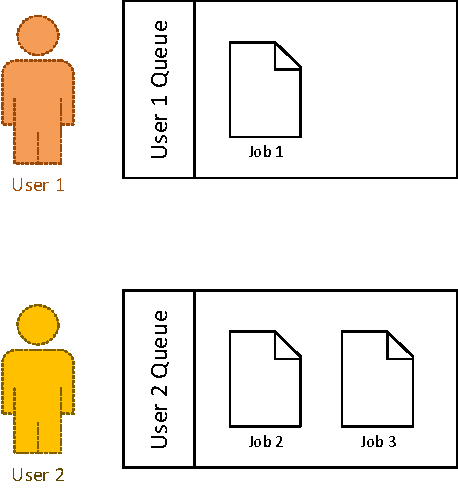
\includegraphics[width=\textwidth]{img/user_job_assignment_order}
		\caption{User 1 receives job 1 while user 2 receives jobs 2 and 3}
		\label{fig:user_job_assignment_order}
	\end{minipage}
	\hfill
	\begin{minipage}[b]{0.45\textwidth}
		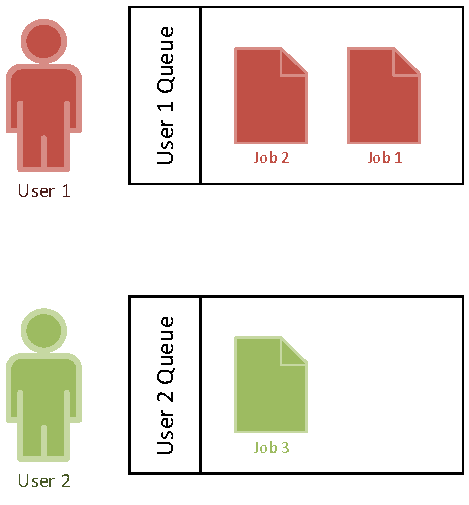
\includegraphics[width=\textwidth]{img/user_job_assignment_order2}
		\caption{User 1 receives jobs 2 and 1 while user 2 receives job 3}
		\label{fig:user_job_assignment_order2}
	\end{minipage}
\end{figure}

\subsecref{subsec:rl_others} outlines three different types of policies (refer to \tabref{tab:rl_others_policies_overview} for a detailed explanation of the policies) that take into account the previously outlined job assignment ordering principle and exploit it in their state space modeling. This is done by means of integrating an additional parameter $B$ that defines how many jobs have to be considered when trying to optimally assign jobs queuing in the global queue to users. This is done by listing all possible combinations by accounting for the job order as well. Refer to \lstref{lst:wz_combinations} for the actual implementation.

\begin{lstlisting}[caption=State space modeling by considering $B$ jobs from the global queue and integrating all possible combinations,label=lst:wz_combinations,style=CustomPython]
	combinations = list(itertools.product(range(self.number_of_users), repeat=self.wait_size))
    for i, combination in enumerate(combinations):
        state_space[i] = a + [p[user_index][job_index] for job_index, user_index in enumerate(combination)]
\end{lstlisting}

This approach effectively simulates batch policies with batch sizes $K>1$.

\glsresetall

\chapter{Empirical Analysis}
\label{ch:empirical_analysis}

\section{Methodology}

In order to consistently and fairly evaluate all policies with the methods defined in the previous chapters, the following methodology was put in place:
\begin{enumerate*}
	\item Each policy has its own simulation script that initializes a process that uses the predefined policy as means to optimally assign jobs to tasks
	\item Parameters are centrally defined
	\item Different \glspl{kpi} have been defined which are used to assert the efficiency of one policy against one another.
\end{enumerate*}

\subsection{Simulation Script}

Each simulation script is the abstract element that imports all required dependencies, initializes the \texttt{SimPy} simulation environment, the statistics file into which the policy dumps all data on runtime, the policy object itself to be used for the assignment and the workflow process to be used. 

The script initializes the chosen workflow process and then calls the tokens generation method of the start event. Eventually the whole simulation is started by calling the run method of the \texttt{SimPy} environment. A snippet of a simulation script can be found in \lstref{lst:simulation_script}.

\begin{lstlisting}[caption=Example of the structure of a simulation script. Here for the K-Batch policy using the \gls{dmf} solver,label=lst:simulation_script,style=CustomPython]
	import simpy
	from evaluation.statistics import calculate_statistics
	from evaluation.subplot_evolution import evolution
	from policies.optimization.batch.k_batch import K_BATCH
	from simulations import *
	from solvers.dmf_solver import dmf

	policy_name = "{}_BATCH_DMF_NU{}_GI{}_SIM{}".format(BATCH_SIZE,NUMBER_OF_USERS, GENERATION_INTERVAL, SEED, SIM_TIME)

	env = simpy.Environment()

	file_policy = create_files("{}.csv".format(policy_name))

	policy = K_BATCH(env, NUMBER_OF_USERS, WORKER_VARIABILITY, file_policy,BATCH_SIZE, dmf)

	start_event = acquisition_process(env,policy,1,GENERATION_INTERVAL,False,None,None,None)

	env.process(start_event.generate_tokens())

	env.run(until=SIM_TIME)

	file_policy.close()

	calculate_statistics(file_policy.name, outfile=True)

	evolution(file_policy.name, outfile=True)
\end{lstlisting}

\subsection{Workflow Process Modeling}

Two different types of processes have been defined:
\begin{enumerate*}
	\item Consisting of only one user task.
	\item A complex workflow process that is modeled against an acquisition process used in the real estate field for the acquisition of real estate properties.
\end{enumerate*}

\figref{fig:simple_process} illustrates the simple process.

\fig[0.5\textwidth]{simple_process}{Simple workflow process consisting of only one user task}{fig:simple_process}

\figref{fig:acquisition_process} illustrates the complex acquisition process.

\fig[\textwidth]{acquisition_process}{Acquisition workflow process consisting of multiple user tasks and decision nodes}{fig:acquisition_process}

\subsection{Global Simulation and Process Parameters Definition}

One key aspect in order to assert comparability across policies while simulated is to centrally define all parameters. \lstref{lst:central_parameters} shows the key central parameters defined as global variables.

\begin{lstlisting}[caption=Global parameters definition that ensures comparability across simulation runs,label=lst:central_parameters,style=CustomPython]
	NUMBER_OF_USERS = 3
	SERVICE_INTERVAL = 1
	GENERATION_INTERVAL = 3
	SIM_TIME = 1000
	BATCH_SIZE = 5
	TASK_VARIABILITY = 0.2 * SERVICE_INTERVAL
	WORKER_VARIABILITY = 0.2 * SERVICE_INTERVAL
	SEED = 2
\end{lstlisting}

\subsection{\glsentryshortpl{kpi} for Asserting Policy's Efficacy and Data Visualization}

Based on \citet{Pinedo2008}'s and \citet{Zeng2005}'s definitions in their works, different \glspl{kpi} have been defined to assert the efficacy of a policy, such as lateness, waiting time, service time, number of tokens completed, user loads and system load. Following the formal definitions of the per token $j$ \glspl{kpi} in respect to lateness $L_j$, wait time $w_j$, service time $p_{ij}$ of assigned user $i$ to token $j$, arrival time $A_j$, assignment time $a_j$, start time $S_j$ and finish time $F_j$.

\begin{align}
	L_j&=F_j-A_j \label{eq:lateness}\\
	w_j&=S_j-A_j \\
	p_{ij}&=F_j-S_j
\end{align}

Moreover, if we account for simulation time $T$, load $l_i$ of user $i$ is defined as the sum of all service times of tokens that have been assigned to him during the simulation divided by the total simulation time $T$, or formally:

\begin{equation}
	l_i=\frac{\sum_j p_{ij}}{T}
\end{equation}

and thus the average system load $\overline{l}$ over all $n$ users participating is defined as the average across all user's loads \ie

\begin{equation}
	\overline{l} = \frac{\sum_i l_i}{n}
\end{equation}

A summary plot with all \glspl{kpi} is done for each simulation script. \figref{fig:kpi_plot} shows an example of how this summary looks like.

\fig[\textwidth]{3_BATCH_MSA_NU2_GI3_SIM50_KPI}{\glsentryfullpl{kpi}  summary plot for a 3-Batch policy using the \glsentryfull{msa} solver, with two users, generation interval set to three and simulation time $T$ set to 50}{fig:kpi_plot}

Additionally, for a more in depth visualization of a policy's performance, an evolution plot is also necessary. All types of policies share a common queues configuration, with a single global queue and a user specific queue. Each policy defines the maximal threshold a specific queue can reach. For a detailed explanation of the queues conformation refer to \secref{sec:opt_policies}.

The evolution plot shows the state change for the policy being analyzed by plotting the flow of a token across different user tasks. \figref{fig:evo_plot} shows such an example.

\fig[\textwidth]{3_BATCH_MSA_NU2_GI3_SIM50_EVO}{Evolution plot for a 3-Batch policy using the \glsentryfull{msa} solver, with two users, generation interval set to three and simulation time $T$ set to 50}{fig:evo_plot}

Finally, when comparing different policies between each other, \citet{Milo2012}'s definition of speedup $S$ between two quantities $q_1$ and $q_2$ is adopted, which he formally defines as:

\begin{equation}
	S=\frac{q_1}{q_2}
\end{equation}

\clearpage

\section{Optimization}
\label{sec:op_results}

This section focuses on the results of the different types of policies using the optimization solvers outlined in \secref{sec:opt_policies}. All simulations have been tested with different combination of global variables \ie number of users, service interval, generation interval, length of simulation time, batch size (where it applies), task variability, worker variability and random state seed (where it applies). For ease of reading purposes, the global variables have been set to the following parameters according to the default column in \tabref{tab:global_parameters_sim}.

% Please add the following required packages to your document preamble:
% \usepackage{booktabs}
\begin{table}[!ht]
\centering
\begin{tabular}{@{}lll@{}}
\toprule
Variable            & Default     & Valid Range \\ \midrule
Number of Users     & $5$           & $1-\infty$      \\
Service Interval    & $1$           & $1-\infty$      \\
Generation Interval & $3$           & $1-\infty$      \\
Simulation Time     & $1000$          & $1-\infty$      \\
Batch Size          & $5$ ($1$ for 1-Batch-1)           & $1-\infty$      \\
Task Varaibility    & $20\%$        & $0\%-100\%$      \\
Worker Variability  & $20\%$        & $0\%-100\%$      \\
Random State Seed   & $2$           & $\emptyset-\infty$      \\
Workflow Process    & Acquisition & Acquisition, Simple      \\ \bottomrule
\end{tabular}
\caption{Global parameters for simulation}
\label{tab:global_parameters_sim}
\end{table}

\subsection{Comparison with Existing Literature}
\label{subsec:opt_comparison}

\citet[pp. 18-22]{Zeng2005} outline in their work how different global parameters configurations and policy usage can affect \glspl{kpi}. They summarize their key findings as follows:
\begin{enumerate*}
	\item Usage of batch optimization should be done only with medium to high system load \citep[p. 24]{Zeng2005}.
	\item Batch optimization policies without a fixed batch size, such as 1-Batch-1 yield best results \citep[p. 24]{Zeng2005}.
\end{enumerate*}

In order to assert the validity of the interpretation of \citet{Zeng2005}'s works and all subsequent derivative policies a comparison with similar configurations has been made for all five optimization policies. \citet{Zeng2005}'s main efficiency parameter is defined as the maximum flowtime or in their own words: ``In business terms, maximum flowtime represents the guaranteed response time across tasks, indicating the quality of services'' \citep[p. 17]{Zeng2005}. In this study, the comparable parameter used to evaluate a policy's efficiency is called lateness and has been previously defined in \equref{eq:lateness}. In regards to lateness, \figref{fig:opt_kpis_comp} shows that akin results to \citet{Zeng2005}'s are obtained.

\fig[\textwidth]{opt_kpis_comp}{\glsentryfullpl{kpi}  comparison for different optimization policies using the \glsentryfull{msa} solver for batch policies}{fig:opt_kpis_comp}  

The simulations have been run with the parameters outlined in \tabref{tab:global_parameters_sim} by using the same solver used by \citet{Zeng2005}: \gls{msa}.

By running the same simulations with the optimization solver implemented for this thesis (\ie \gls{st}, refer to \secref{sec:opt_policies}), ceteris paribus, the summarized \glspl{kpi} amongst all optimization policies can be seen in \figref{fig:opt_st_kpis_comp}.

\fig[\textwidth]{opt_st_kpis_comp}{\glsentryfullpl{kpi}  comparison for different optimization policies using the \glsentryfull{st} solver for batch policies}{fig:opt_st_kpis_comp}

The percent speedup for both batch policies with a higher batch size is tiny, but when considering the speedup between the 1-Batch-1 policy with \gls{msa} and \gls{st}, a wealthy speedup is present for all \glspl{kpi}. For a detailed overview of the overall speedups of the \gls{st} against the \gls{msa} solver refer to \figref{fig:opt_kpis_comp_gain}.

\fig[\textwidth]{opt_kpis_comp_gain}{\glsentryfullpl{kpi}  speedup comparison between the \glsentryfull{msa} and the \glsentryfull{st} solvers for 5-Batch, 5-Batch-1 and 1-Batch-1}{fig:opt_kpis_comp_gain}

Astonishing speedups have been observed for the 1-Batch-1 policy, which is indeed the most efficient policy as mentioned by \citet{Zeng2005} (for a detailed comparison of how different batch sizes affect the policy's \glspl{kpi} refer to \subsecref{subsec:kbatch_bscomp_app} and \subsecref{subsec:kbatchone_bscomp_app}) \citep[p. 24]{Zeng2005}. \tabref{tab:opt_kpis_comp_gain} summarizes these values.

% Please add the following required packages to your document preamble:
% \usepackage{booktabs}
\begin{table}[!ht]
\centering
\begin{tabular}{@{}ll@{}}
\toprule
\gls{kpi}                 & Speedup \\ \midrule
Lateness            & $1.23$             \\
Wait Time           & $4.0$             \\
Service Time        & $1.1$             \\
Average System Load & $1.1$             \\ \bottomrule
\end{tabular}
\caption{Speedup across all \glsentryfullpl{kpi} of the \glsentryfull{st} against the \glsentryfull{msa} solver}
\label{tab:opt_kpis_comp_gain}
\end{table}

\clearpage

\section{\glsentrylong{rl}}
\label{sec:rl_results}

This section focuses on the results obtained with the \gls{rl} methods outlined in \secref{sec:rl_policies}. A more in-depth review of the different policies is required, thus a finer subdivision has been made in different subsections per policy type: \subsecref{subsec:rl_batch} focuses on batch policies, \subsecref{subsec:rl_llqp} focuses on \gls{llqp} policies and \subsecref{subsec:rl_others} focuses on all remaining policies that do not fit in either of the previous categories.

In order to maintain fairness amongst \gls{rl} training methods, all required parameters are globally set and equal across all simulation scripts and can be found summarized in \tabref{tab:global_rl_params} which complement the global simulation parameters depicted in \tabref{tab:global_parameters_sim}.

% Please add the following required packages to your document preamble:
% \usepackage{booktabs}
\begin{table}[!ht]
\centering
\begin{tabular}{@{}ll@{}}
\toprule
Parameter        & Value  \\ \midrule
Discount factor $\gamma$            & $0.5$    \\
Step size parameter $\alpha$            & $0.0001$ \\
\gls{ep} threshold $\epsilon$          & $0.1$    \\
\gls{mc} epochs        & $1000$   \\
\glspl{ann} \gls{mc} epochs & $10000$ \\
\gls{mc} and \glspl{ann} \gls{mc} epoch training time & $100$ \\
\gls{td} training time & $100000$   \\ \bottomrule
\end{tabular}
\caption{Global \glsentryfull{rl} parameters}
\label{tab:global_rl_params}
\end{table}

Comparisons will be made, where not otherwise stated, with the corresponding optimization policy simulated under the same conditions.

\subsection{Batch}
\label{subsec:rl_batch}

Five different batch policies with \gls{rl} have been developed. \tabref{tab:rl_batch_policies_overview} gives an overview.

% Please add the following required packages to your document preamble:
% \usepackage{booktabs}
% \usepackage{graphicx}
\begin{table}[!ht]
\centering
\resizebox{\textwidth}{!}{%
\begin{tabular}{@{}lllll@{}}
\toprule
Technical Name          & Policy Type & Update Method & $Q$ Value Method               & Other Characteristics     \\ \midrule
k\_batch\_mc\_vfa       & 1-Batch     & \gls{mc}            & \gls{vfa} & None                      \\
k\_batch\_mc\_vfa\_op   & 1-Batch     & \gls{mc}            & \gls{vfa} & \gls{op}                \\
k\_batch\_mc\_vfa\_opep & 1-Batch     & \gls{mc}            & \gls{vfa} & \gls{ep}, \gls{op} \\
k\_batch\_td\_vfa\_op   & 1-Batch     & \gls{td}            & \gls{vfa} & \gls{op}                \\
k\_batchone\_td\_vfa\_op   & 1-Batch-1     & \gls{td}            & \gls{vfa} & \gls{op}                \\ \bottomrule
\end{tabular}%
}
\caption{Overview of developed batch policies with \glsentryfull{rl}}
\label{tab:rl_batch_policies_overview}
\end{table}

\tabref{tab:rl_batch_kpis_comp_gain} summarizes the results. For the detailed results refer to \subsecref{subsec:onebatch_rl_msa_comp_app} for 1-Batch respectively to \subsecref{subsec:onebatchone_rl_msa_comp_app} for 1-Batch-1.

% Please add the following required packages to your document preamble:
% \usepackage{booktabs}
% \usepackage{graphicx}
\begin{table}[!ht]
\centering
\resizebox{\textwidth}{!}{%
\begin{tabular}{@{}llllll@{}}
\toprule
\gls{kpi}                 & k\_batch\_mc\_vfa & k\_batch\_mc\_vfa\_op & k\_batch\_mc\_vfa\_opep & k\_batch\_td\_vfa\_op & k\_batchone\_td\_vfa\_op \\ \midrule
Lateness            & $1.22$                  & $1.24$                      & $1.22$                        & $1.23$                      & $1.23$                         \\
Wait Time           & $2.63$                  & $3.08$                      & $2.39$                        & $3.62$                      & $3.51$                         \\
Service Time        & $1.11$                  & $1.11$                      & $1.12$                        & $1.1$                      & $1.1$                         \\
Average System Load & $1.11$                  & $1.11$                      & $1.12$                        & $1.1$                      & $1.1$                         \\ \bottomrule
\end{tabular}%
}
\caption{Speedup across all \glsentryfullpl{kpi} of the batch policies with \glsentryfull{rl} against the \glsentryfull{msa} solver}
\label{tab:rl_batch_kpis_comp_gain}
\end{table}

\subsection{\glsentrylong{llqp}}
\label{subsec:rl_llqp}

Three different \gls{llqp} policies with \gls{rl} have been developed. \tabref{tab:rl_llqp_policies_overview} gives an overview. Other policies have been implemented for evaluating different \gls{rl} methods, however they are not considered for the final evaluation. These policies can be seen in \tabref{tab:rl_llqp_add_policies_overview}.

% Please add the following required packages to your document preamble:
% \usepackage{booktabs}
% \usepackage{graphicx}
\begin{table}[!ht]
\centering
\resizebox{\textwidth}{!}{%
\begin{tabular}{@{}lllll@{}}
\toprule
Technical Name          & Policy Type & Update Method & $Q$ Value Method               & Other Characteristics     \\ \midrule
llqp\_mc\_vfa\_op       & \gls{llqp}     & \gls{mc}            & \gls{vfa} & \gls{op}                      \\
llqp\_td\_vfa\_op   & \gls{llqp}     & \gls{td}            & \gls{vfa} & \gls{op}                \\
llqp\_td\_tf\_op   & \gls{llqp}     & \gls{td}            & \glspl{ann} & \gls{op}, \gls{1l}                \\ \bottomrule
\end{tabular}%
}
\caption{Overview of developed \glsentryfull{llqp} policies with \glsentryfull{rl}}
\label{tab:rl_llqp_policies_overview}
\end{table}

\tabref{tab:rl_llqp_kpis_comp_gain} shows the summarized results. For the detailed results refer to \subsecref{subsec:llqp_rl_msa_comp_app}.

% Please add the following required packages to your document preamble:
% \usepackage{booktabs}
\begin{table}[!ht]
\centering
\begin{tabular}{@{}llll@{}}
\toprule
\gls{kpi}                 & llqp\_mc\_vfa\_op & llqp\_td\_vfa\_op & llqp\_td\_tf\_op \\ \midrule
Lateness            & $1.0$                  & $1.0$                  & $1.0$                 \\
Wait Time           & $0.92$                  & $0.99$                  & $1.02$                 \\
Service Time        & $1.01$                  & $1.0$                  & $1.0$                 \\
Average System Load & $1.01$                  & $1.0$                  & $1.0$                 \\ \bottomrule
\end{tabular}
\caption{Speedup across all \glsentryfullpl{kpi} of the \glsentryfull{llqp} policies with \glsentryfull{rl} against the \glsentryfull{msa} solver}
\label{tab:rl_llqp_kpis_comp_gain}
\end{table}

\tabref{tab:llqp_mc_vfa_op_vs_on} shows the comparison between \gls{op} and \gls{onp} approaches.

% Please add the following required packages to your document preamble:
% \usepackage{booktabs}
\begin{table}[!ht]
\centering
\begin{tabular}{@{}llll@{}}
\toprule
\gls{kpi}                 & llqp\_mc\_vfa\_op & llqp\_mc\_vfa & Speedup \\ \midrule
Lateness            & $1.2756$                  & $1.2914$              & $0.99$                   \\
Wait Time           & $0.0796$                  & $0.0711$              & $1.12$                   \\
Service Time        & $1.1960$                  & $1.2203$              & $0.98$                   \\
Average System Load & $38.22\%$                  & $39.00\%$              & $0.98$                   \\ \bottomrule
\end{tabular}
\caption{\glsentryfullpl{kpi} comparison between \glsentryfull{op} and \glsentryfull{onp} approaches}
\label{tab:llqp_mc_vfa_op_vs_on}
\end{table}

\subsection{Others}
\label{subsec:rl_others}

Three different additional policies with \gls{rl} have been developed which have been used to fully emulate the behavior of K-Batch and 1-Batch-1 (as explained in \subsecref{subsec:batch_size_emulation}). \tabref{tab:rl_others_policies_overview} gives an overview.

% Please add the following required packages to your document preamble:
% \usepackage{booktabs}
% \usepackage{graphicx}
\begin{table}[!ht]
\centering
\resizebox{\textwidth}{!}{%
\begin{tabular}{@{}lllll@{}}
\toprule
Technical Name          & Policy Type & Update Method & $Q$ Value Method               & Other Characteristics     \\ \midrule
wz\_td\_vfa\_op       & \gls{wz}     & \gls{td}            & \gls{vfa} & \gls{op}                      \\
wz\_one\_td\_vfa\_op   & \gls{wzo}     & \gls{td}            & \gls{vfa} & \gls{op}                \\
bi\_one\_mc\_tf   & \gls{bi}     & \gls{mc}            & \glspl{ann} & \gls{pg}                \\ \bottomrule
\end{tabular}%
}
\caption{Overview of additional developed policies with \glsentryfull{rl}}
\label{tab:rl_others_policies_overview}
\end{table}

\tabref{tab:rl_others_kpis_comp_gain} shows the summarized results. For the detailed results refer to \subsecref{subsec:others_rl_msa_comp_app}.

% Please add the following required packages to your document preamble:
% \usepackage{booktabs}
% \usepackage{graphicx}
\begin{table}[!ht]
\centering
\resizebox{\textwidth}{!}{%
\begin{tabular}{@{}lllllll@{}}
\toprule
KPI                 & wz\_td\_vfa\_op & wz\_one\_td\_vfa\_op & bi\_one\_mc\_tf\_1l & bi\_one\_mc\_tf\_2l & bi\_one\_mc\_tf\_3l & bi\_one\_mc\_tf\_4l \\ \midrule
Lateness            & $0.97$                & $1.2$                     & $1.07$                    & $0.9$                    & $0.84$                    & $0.84$                    \\
Wait Time           & $0.89$                & $2.33$                     & $2.46$                    & $1.11$                    & $0.85$                    & $0.86$                    \\
Service Time        & $1.21$                & $1.1$                     & $0.98$                    & $0.87$                    & $0.84$                    & $0.84$                    \\
Average System Load & $1.22$                & $1.1$                     & $0.98$                    & $0.87$                    & $0.84$                    & $0.84$                    \\ \bottomrule
\end{tabular}%
}
\caption{Speedup across all \glsentryfullpl{kpi} of the additional policies with \glsentryfull{rl} against the \glsentryfull{msa} solver}
\label{tab:rl_others_kpis_comp_gain}
\end{table}

\section{Discussion}

\subsection{Optimization}
\label{subsec:optimization_discussion}

Using mathematical optimization to solve the assignment problem proves to be an efficient measure, however different solvers yield different solutions and computational complexities. \citet[p. 15]{Zeng2005} mention that \gls{msa} greatly simplifies \gls{dmf} since only those tasks that are immediately available are considered. This consideration is done since the \gls{dmf} problem proves to be computationally expensive to solve \citep[p. 13]{Zeng2005},\citep{Garey1990}. \citet[p. 13]{Zeng2005} propose however that by introducing auxiliary variables one can reduce the complexity of \gls{dmf} and effectively solving it. This is what has been done in this thesis, as outlined in \secref{sec:opt_policies} by introducing new types of solvers. The \gls{st} ``flagship'' solver significantly outperforms the \gls{msa} solver (refer to \figref{fig:k_batchone_st_opt_kpis_comp}). Having said that, the higher computational complexity of \gls{st} compared to \gls{msa} (see \tabref{tab:big_oh_solvers}) questions the practical use of this solver over the other methods. A speedup factor of $1.23$ in respect to lateness requiring a quadratic higher computational complexity poses a dubious trade-off from a business perspective.

\fig[\textwidth]{k_batchone_st_opt_kpis_comp}{\glsentryfullpl{kpi} speedup comparison between \glsentryfull{msa} and \glsentryfull{st} solvers for 1-Batch-1}{fig:k_batchone_st_opt_kpis_comp}

Yet another aspect mentioned by \citet[pp. 17-18]{Zeng2005} is a more ``social'' aspect: the fairness of a policy \ie how fairly are single users treated by a policy during job assignment. \figref{fig:msa_fairness} and \figref{fig:st_fairness} both show how fairly are users treated in the same scenario by the two solvers.

\begin{figure}[!ht]
	\centering
	\begin{minipage}[b]{0.45\textwidth}
		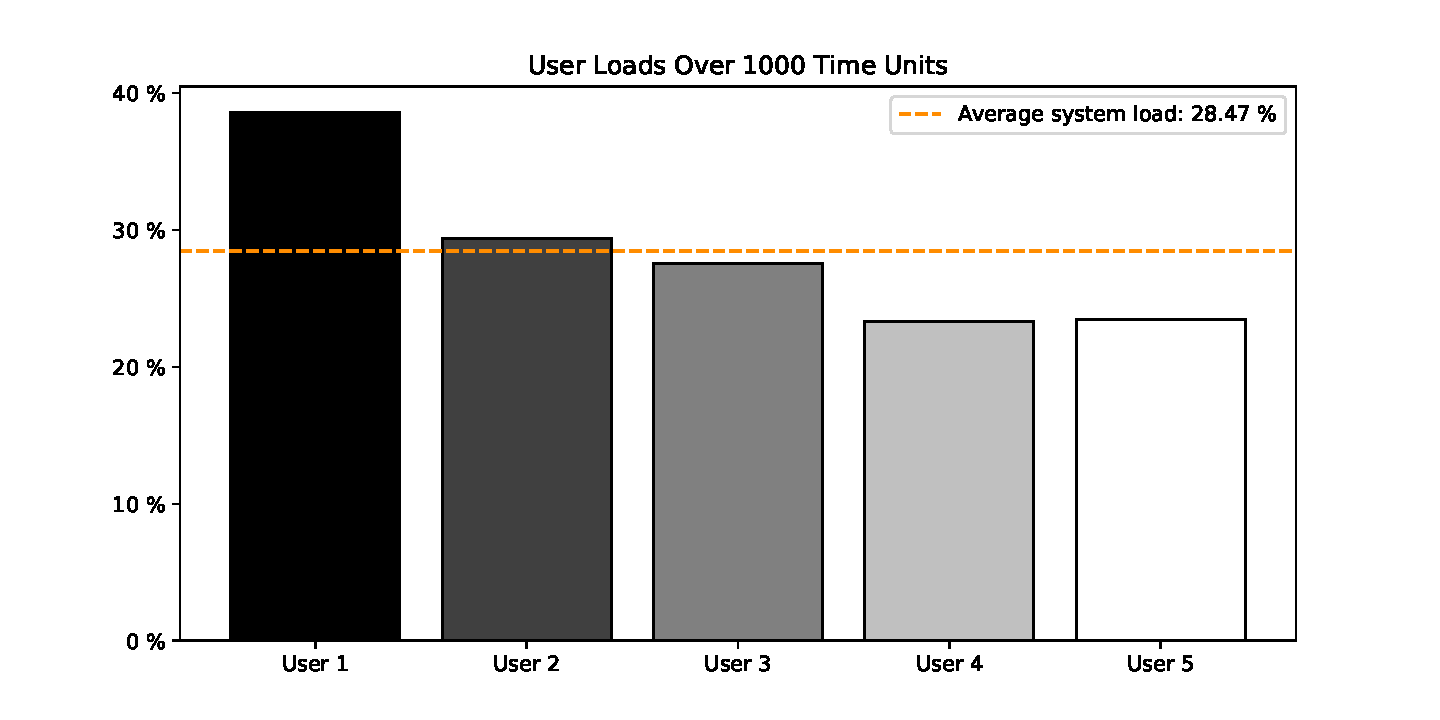
\includegraphics[width=\textwidth]{img/1_BATCHONE_MSA_NU5_GI3_SIM1000_FAIR}
		\caption{User loads distribution for 1-Batch-1 using \glsentryfull{msa}}
		\label{fig:msa_fairness}
	\end{minipage}
	\hfill
	\begin{minipage}[b]{0.45\textwidth}
		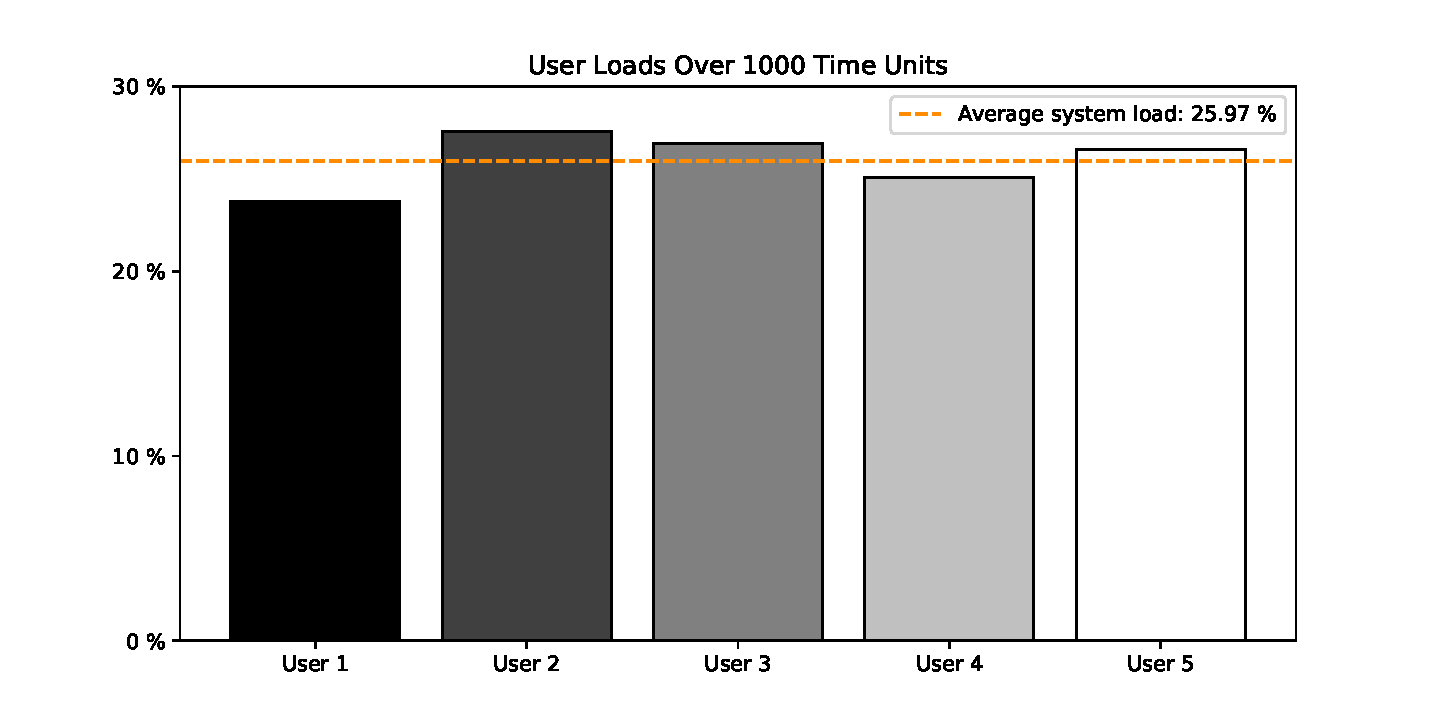
\includegraphics[width=\textwidth]{img/1_BATCHONE_ST_NU5_GI3_SIM1000_FAIR}
		\caption{User loads distribution for 1-Batch-1 using \glsentryfull{st}}
		\label{fig:st_fairness}
	\end{minipage}
\end{figure}

It is clear that \gls{st} is ``fairer'' at balancing loads across users compared to \gls{msa}. 

\subsection{\glsentrylong{rl}}
\label{subsec:rl_discussion}

Let us first focus on \gls{llqp}, which, as explained in \secref{sec:opt_policies}, focuses on assigning a job to the least loaded qualified person. By comparing the results obtained with \gls{rl} against the optimization method, we clearly see that speedups across all \glspl{kpi} are imperceptible (refer to \subsecref{subsec:llqp_rl_msa_comp_app} for more details). This sheds light on two key aspects:
\begin{enumerate*}
	\item \gls{llqp} policies are intrinsically optimized by their nature of implementation.
	\item \gls{rl} methods converge really well (for a $1000$ time steps \gls{llqp} simulation, \gls{llqp} with \gls{td} and \gls{tf} only needs 20 times the simulation time as training in order to perfectly converge to actual \gls{llqp}) and, even if only slightly, exploit internal mechanisms of \gls{llqp} policies to extract better results.
\end{enumerate*}

On the other hand, batch policies exhibit a much bigger optimization potential for which \gls{rl} methods do really adapt well. Lateness speedup of factor $1.24$ for 1-Batch (see \subsecref{subsec:onebatch_rl_msa_comp_app}) respectively $1.23$ for 1-Batch-1 (see \subsecref{subsec:onebatchone_rl_msa_comp_app}) confirm the previous claim.

Lastly, when accounting for job order during assignment (refer to \subsecref{subsec:batch_size_emulation} for the detailed explanation), improvements are observed only under specific conditions:
\begin{enumerate*}
	\item by using \gls{wzo} (see \figref{fig:wz_one_td_vfa_op}) and 
	\item \glspl{ann} with \gls{1l} (see \figref{fig:bi_one_mc_tf_1l} for \glspl{kpi} comparison against \gls{msa} and fig for the graphical representation of the \gls{ann} implemented with \gls{tf}).
\end{enumerate*}

Having said that, deep \glspl{ann} exhibits worse results compared to their equivalent emulated optimization methods. This can be explained from a twofold perspective:
\begin{enumerate*}
	\item \gls{vgp} and
	\item \gls{egp}.
\end{enumerate*}

In brief, \gls{vgp} states that even very large changes in partial derivatives on initial layers have imperceptible effects on subsequent layers \citep{Bengio1994} and \gls{egp} states that huge spikes in the norm of changes in partial derivatives which could potentially grow exponentially can happen under training, thus influencing internal parameters \citep{Bengio1994,Pascanu2012}.

Yet another crucial aspect to consider when undergoing \gls{rl} methods is usage between \gls{onp} or \gls{op} learning (refer to \subsecref{subsec:onpol_pred} for \gls{onp} respectively to \subsecref{subsec:offpol_methods} for \gls{op} \subsecref{subsec:onpol_control}). As shown in \tabref{tab:llqp_mc_vfa_op_vs_on} (and \figref{fig:llqp_mc_vfa_on_vs_off}), \gls{op} methods converge slightly better compared to \gls{onp}, however the change is imperceptible and can be found in different factors (\eg random state seed choice or length of simulation). Having said that, it is important to note that these different approaches are being currently heavily studied by pioneers and the debate is still open, as \citet[pp. 245-249]{Sutton2017} explain in their book. The current key takeaways from this outgoing debate can be summarized as follows \citep{Sutton2017}:
\begin{enumerate*}
	\item Learning \gls{op}
	\item Usage of scalable function approximation methods like linear semi-gradient 
	\item Usage of bootstrapping which is used in \gls{td} methods.
\end{enumerate*}

The combination of all these three factors is referred as ``the deadly triad'' \citep[p. 249]{Sutton2017}. \citet[p. 249]{Sutton2017} argue that dangers can arise only when all three aspects are present, if used singularly convergence properties are safe.

On a more general note, different comparisons have shown huge spikes in speedup of waiting time (\eg \subsecref{subsec:onebatch_rl_msa_comp_app}). Even though compelling, the practical usage is limited: when considering workflow processes with fixed available resources (\ie users participating), huge speedup in job waiting times does not always correlate with better system performance, since it might be the case that even if a job is ready to be assigned there are no available resources to complete such job.

\fig[\textwidth]{llqp_mc_vfa_on_vs_off}{\glsentryfullpl{kpi} comparison between \glsentryfull{op} and \glsentryfull{onp} approaches}{fig:llqp_mc_vfa_on_vs_off}

\glsresetall

\chapter{Conclusion}
\label{ch:conclusion}

\section{Summary}

This thesis' focus was analyzing different approaches for optimally allocating resources inside workflow processes by means of different methods.

Initially, a through literature review has been made in order to establish the existing optimization solution (\ie foundations set by \citet{Zeng2005}), then a roadmap on how to further develop such methods has been laid out. The roadmap encloses a twofold approach:

\begin{enumerate}[label=\textbf{A. \Roman*},ref=Approach \Roman*]
 	\item Further develop mathematical optimizations \label{itm:math_opt}
 	\item Use \gls{rl} methods as novel solution for optimal job assignment. \label{itm:novel_rl}
 \end{enumerate} 

Subsequently, a discrete event simulation environment as outlined in \subsecref{subsec:discrete_event_sim} has been implemented which served as foundation for evaluating all future optimization policies.

For \ref{itm:math_opt} five existing optimization policies as outlined in \secref{sec:opt_policies} have been implemented and evaluated against the existing policies defined by \citet[pp. 13-14]{Zeng2005}. Furthermore, for \ref{itm:novel_rl} a profound literature review about \gls{rl} had to be made and following on the theoretical foundations laid (see \secref{sec:rl_theory}) novel policies for solving the assignment problem based on \gls{rl} have been implemented (see \secref{sec:rl_policies}). Lastly, all \gls{rl} policies have been also evaluated and a comparison between them and the corresponding optimization methods has been made.

\section{Resulting Conclusions}

Optimization methods are viable solutions for optimally assigning jobs to users inside workflow processes, as already argued by \citet{Zeng2005}. Further developed policies relying on mathematical optimization done for this thesis proved indeed to yield better results (see \subsecref{subsec:opt_comparison}), however the higher required complexity (refer to \subsecref{subsec:optimization_discussion}) poses a critical trade-off. \ref{rq:one} can be affirmatively answer: there is definitely potential for further development and optimization of existing methods but further questions arise:

\begin{enumerate}[label=\textbf{Q. \Roman*}]
	\item Does a slight increase in performance justify the higher computational requirements?
	\item Can only one \gls{kpi} be chosen as central parameter to evaluate a policy's performance or is a combination of different \glspl{kpi} more suitable?
	\item Is it always the best solution to use only one type of optimizer or is it better to follow a more flexible approach and chose different policies on a per case basis?
\end{enumerate}

All these questions must be accounted for when considering policy based optimization in workflow processes integration in IT governance.

On the other hand, \gls{rl} methods demonstrate to overcome some of the problematics laid by optimization very well:
\begin{enumerate*}
	\item Generally less computationally expensive
	\item Can be adopted relatively fast
	\item Are generally more ``dynamic'' and can adapt and exploit case specific characteristics.
\end{enumerate*}

Then again \gls{rl} methods are not exempt from disadvantages:
\begin{enumerate*}
	\item They require long training sessions in order to equal (or even outperform) optimization methods
	\item When using \glspl{ann}, overfitting might lead to suboptimal solution in which policies get stuck (for viable solutions refer to \citet{Srivastava2014})
	\item Multilayer \glspl{ann} (\ie deep \glspl{ann}) are very sensitive to \gls{vgp} and \gls{egp} \citep{Bengio1994,Pascanu2012}.
\end{enumerate*}

In general \gls{rl} based approaches are a refreshing and novel methodology for solving optimization problems but require further development and sound domain knowledge.

\section{Outlook}

This thesis does a first step in laying the foundations for viable alternatives to existing optimization techniques for workflow processes. A direct follow up consists in testing in operative environments the introduction feasibility and efficiency measured in the simulation environment outlined in this thesis. This includes testing the robustness, efficacy and viability of the proposed policies by putting them under ``real-world'' stress situation in order to assert the efficiency claims. For \gls{rl} methods executing lengthy training sessions might prove impractical: thousands of training sessions required by \gls{rl} methods in order to comply with convergence properties can prove infeasible for companies that are not able to generate such amounts of data, thus directly limiting applicability of these methods.

\gls{rl} is a novel field that is currently still being actively researched and pursued, as it has yield promising results \citep{Mnih2015,Silver2016}. By using \glspl{ann} one can effectively approximate nonlinear functions as it has been outlined in \subsecref{subsubsec:ann_theory}. Even though in this thesis only feedforward \glspl{ann} have been used, the problem domain is very well suited for the recurrent variant as well.

Moreover, bleeding edge domains have originated from \gls{rl} such as \gls{irl} \citep{Ng2000} and \gls{al} which is based on the former \citep{Abbeel2004}. \gls{al} could prove to be yet another captivating approach to solve the assignment problem in which the reward function is not explicitly modeled, instead an ``expert'' of the domain (\ie a mathematical solver such as \gls{msa}) demonstrates a task and by means of \gls{al} the policy is trained \citep{Abbeel2004}.

Having said that, \ref{rq:two} can be answered positively as well: there are indeed state of the art approaches that can be used as alternatives or complements to the job assignment mathematical optimization. 

\appendix

\glsresetall

\chapter{Literature Overview}

\fig[\textwidth]{literature_brainstorm}{Literature per topic categorization overview}{fig:literature_brainstorm}

\clearpage

\glsresetall

\chapter{Optimization Results}

\section{\glsentrylong{llqp}}

\subsection{\glsentryshortpl{kpi}}
\label{subsec:llqp_kpi_app}

\fig[\textwidth]{llqp_res/LLQP_NU5_GI3_SIM1000_KPI}{\glsentryfull{llqp} \glsentryfullpl{kpi}}{fig:LLQP_NU5_GI3_SIM1000_KPI}

\clearpage

\section{\glsentrylong{sq}}

\subsection{\glsentryshortpl{kpi}}
\label{subsec:sq_kpi_app}

\fig[\textwidth]{sq_res/SQ_NU5_GI3_SIM1000_KPI}{\glsentryfull{sq} \glsentryfullpl{kpi}}{fig:SQ_NU5_GI3_SIM1000_KPI}

\clearpage

\section{K-Batch}

\subsection{\glsentryshortpl{kpi}}
\label{subsec:kbatch_kpi_app}

\fig[\textwidth]{kbatch_res/5_BATCH_MSA_NU5_GI3_SIM1000_KPI}{K-Batch with \glsentryfull{msa} \glsentryfullpl{kpi}}{fig:5_BATCH_MSA_NU5_GI3_SIM1000_KPI}
\fig[\textwidth]{kbatch_res/5_BATCH_DMF_NU5_GI3_SIM1000_KPI}{K-Batch with \glsentryfull{dmf} \glsentryfullpl{kpi}}{fig:5_BATCH_DMF_NU5_GI3_SIM1000_KPI}
\fig[\textwidth]{kbatch_res/5_BATCH_SDMF_NU5_GI3_SIM1000_KPI}{K-Batch with \glsentryfull{sdmf} \glsentryfullpl{kpi}}{fig:5_BATCH_SDMF_NU5_GI3_SIM1000_KPI}
\fig[\textwidth]{kbatch_res/5_BATCH_ESDMF_NU5_GI3_SIM1000_KPI}{K-Batch with \glsentryfull{esdmf} \glsentryfullpl{kpi}}{fig:5_BATCH_ESDMF_NU5_GI3_SIM1000_KPI}
\fig[\textwidth]{kbatch_res/5_BATCH_ST_NU5_GI3_SIM1000_KPI}{K-Batch with \glsentryfull{st} \glsentryfullpl{kpi}}{fig:5_BATCH_ST_NU5_GI3_SIM1000_KPI}

\clearpage

\subsection{Batch Sizes Comparison}
\label{subsec:kbatch_bscomp_app}

\fig[\textwidth]{kbatch_res/1-5_BATCH_MSA_NU5_GI3_SIM1000_BSEVAL}{K-Batch with \glsentryfull{msa} batch size comparison}{fig:1-5_BATCH_MSA_NU5_GI3_SIM1000_BSEVAL}
\fig[\textwidth]{kbatch_res/1-5_BATCH_ST_NU5_GI3_SIM1000_BSEVAL}{K-Batch with \glsentryfull{st} batch size comparison}{fig:1-5_BATCH_ST_NU5_GI3_SIM1000_BSEVAL}

\clearpage

\section{K-Batch-1}

\subsection{\glsentryshortpl{kpi}}
\label{subsec:kbatchone_kpi_app}

\fig[\textwidth]{kbatchone_res/5_BATCHONE_MSA_NU5_GI3_SIM1000_KPI}{K-Batch-1 with \glsentryfull{msa} \glsentryfullpl{kpi}}{fig:5_BATCHONE_MSA_NU5_GI3_SIM1000_KPI}
\fig[\textwidth]{kbatchone_res/5_BATCHONE_DMF_NU5_GI3_SIM1000_KPI}{K-Batch-1 with \glsentryfull{dmf} \glsentryfullpl{kpi}}{fig:5_BATCHONE_DMF_NU5_GI3_SIM1000_KPI}
\fig[\textwidth]{kbatchone_res/5_BATCHONE_SDMF_NU5_GI3_SIM1000_KPI}{K-Batch-1 with \glsentryfull{sdmf} \glsentryfullpl{kpi}}{fig:5_BATCHONE_SDMF_NU5_GI3_SIM1000_KPI}
\fig[\textwidth]{kbatchone_res/5_BATCHONE_ESDMF_NU5_GI3_SIM1000_KPI}{K-Batch-1 with \glsentryfull{esdmf} \glsentryfullpl{kpi}}{fig:5_BATCHONE_ESDMF_NU5_GI3_SIM1000_KPI}
\fig[\textwidth]{kbatchone_res/5_BATCHONE_ST_NU5_GI3_SIM1000_KPI}{K-Batch-1 with \glsentryfull{st} \glsentryfullpl{kpi}}{fig:5_BATCHONE_ST_NU5_GI3_SIM1000_KPI}

\clearpage

\subsection{Batch Sizes Comparison}
\label{subsec:kbatchone_bscomp_app}

\fig[\textwidth]{kbatchone_res/1-5_BATCHONE_MSA_NU5_GI3_SIM1000_BSEVAL}{K-Batch-1 with \glsentryfull{msa} batch size comparison}{fig:1-5_BATCHONE_MSA_NU5_GI3_SIM1000_BSEVAL}
\fig[\textwidth]{kbatchone_res/1-5_BATCHONE_ST_NU5_GI3_SIM1000_BSEVAL}{K-Batch-1 with \glsentryfull{st} batch size comparison}{fig:1-5_BATCHONE_ST_NU5_GI3_SIM1000_BSEVAL}

\clearpage

\section{1-Batch-1}

\subsection{\glsentryshortpl{kpi}}
\label{subsec:onebatchone_kpi_app}

\fig[\textwidth]{onebatchone_res/1_BATCHONE_MSA_NU5_GI3_SIM1000_KPI}{1-Batch-1 with \glsentryfull{msa} \glsentryfullpl{kpi}}{fig:1_BATCHONE_MSA_NU5_GI3_SIM1000_KPI}
\fig[\textwidth]{onebatchone_res/1_BATCHONE_DMF_NU5_GI3_SIM1000_KPI}{1-Batch-1 with \glsentryfull{dmf} \glsentryfullpl{kpi}}{fig:1_BATCHONE_DMF_NU5_GI3_SIM1000_KPI}
\fig[\textwidth]{onebatchone_res/1_BATCHONE_SDMF_NU5_GI3_SIM1000_KPI}{1-Batch-1 with \glsentryfull{sdmf} \glsentryfullpl{kpi}}{fig:1_BATCHONE_SDMF_NU5_GI3_SIM1000_KPI}
\fig[\textwidth]{onebatchone_res/1_BATCHONE_ESDMF_NU5_GI3_SIM1000_KPI}{1-Batch-1 with \glsentryfull{esdmf} \glsentryfullpl{kpi}}{fig:1_BATCHONE_ESDMF_NU5_GI3_SIM1000_KPI}
\fig[\textwidth]{onebatchone_res/1_BATCHONE_ST_NU5_GI3_SIM1000_KPI}{1-Batch-1 with \glsentryfull{st} \glsentryfullpl{kpi}}{fig:1_BATCHONE_ST_NU5_GI3_SIM1000_KPI}

\clearpage

\glsresetall

\chapter{\glsentrylong{rl} Results}

\section{1-Batch}

\subsection{\glsentryshortpl{kpi}}
\label{subsec:onebatch_rl_kpi_app}

\fig[\textwidth]{kbatch_rl_res/1_BATCH_MC_VFA_NU5_GI3_SIM1000_KPI}{1-Batch with \glsentryfull{mc} and \glsentryfull{vfa} \glsentryfullpl{kpi}}{fig:1_BATCH_MC_VFA_NU5_GI3_SIM1000_KPI}
\fig[\textwidth]{kbatch_rl_res/1_BATCH_MC_VFA_OP_NU5_GI3_SIM1000_KPI}{1-Batch with \glsentryfull{mc}, \glsentryfull{vfa} and \glsentryfull{op} \glsentryfullpl{kpi}}{fig:1_BATCH_MC_VFA_OP_NU5_GI3_SIM1000_KPI}
\fig[\textwidth]{kbatch_rl_res/1_BATCH_MC_VFA_OPEP_NU5_GI3_SIM1000_KPI}{1-Batch with \glsentryfull{mc}, \glsentryfull{vfa}, \glsentryfull{op} and \glsentryfull{ep} \glsentryfullpl{kpi}}{fig:1_BATCH_MC_VFA_OPEP_NU5_GI3_SIM1000_KPI}
\fig[\textwidth]{kbatch_rl_res/1_BATCH_TD_VFA_OP_NU5_GI3_TRSD2_SIM1000_KPI}{1-Batch with \glsentryfull{td}, \glsentryfull{vfa} and \glsentryfull{op} \glsentryfullpl{kpi}}{fig:1_BATCH_TD_VFA_OP_NU5_GI3_TRSD2_SIM1000_KPI}

\clearpage

\subsection{Comparison with \glsentryshort{msa}}
\label{subsec:onebatch_rl_msa_comp_app}

\fig[\textwidth]{kbatch_rl_res/k_batch_mc_vfa}{1-Batch with \glsentryfull{mc} and \glsentryfull{vfa} \glsentryfull{msa} comparison}{fig:k_batch_mc_vfa}
\fig[\textwidth]{kbatch_rl_res/k_batch_mc_vfa_op}{1-Batch with \glsentryfull{mc}, \glsentryfull{vfa} and \glsentryfull{op} \glsentryfull{msa} comparison}{fig:k_batch_mc_vfa_op}
\fig[\textwidth]{kbatch_rl_res/k_batch_mc_vfa_opep}{1-Batch with \glsentryfull{mc}, \glsentryfull{vfa}, \glsentryfull{op} and \glsentryfull{ep} \glsentryfull{msa} comparison}{fig:k_batch_mc_vfa_opep}
\fig[\textwidth]{kbatch_rl_res/k_batch_td_vfa_op}{1-Batch with \glsentryfull{td}, \glsentryfull{vfa} and \glsentryfull{op} \glsentryfull{msa} comparison}{fig:k_batch_td_vfa_op}

\clearpage

\section{1-Batch-1}

\subsection{\glsentryshortpl{kpi}}
\label{subsec:onebatchone_rl_kpi_app}

\fig[\textwidth]{kbatchone_rl_res/1_BATCHONE_TD_VFA_OP_NU5_GI3_TRSD2_SIM1000_KPI}{1-Batch-1 with \glsentryfull{td}, \glsentryfull{vfa} and \glsentryfull{op} \glsentryfullpl{kpi}}{fig:1_BATCHONE_TD_VFA_OP_NU5_GI3_TRSD2_SIM1000_KPI}

\clearpage

\subsection{Comparison with \glsentryshort{msa}}
\label{subsec:onebatchone_rl_msa_comp_app}

\fig[\textwidth]{kbatchone_rl_res/k_batchone_td_vfa_op}{1-Batch-1 with \glsentryfull{td}, \glsentryfull{vfa} and \glsentryfull{op} \glsentryfull{msa} comparison}{fig:k_batchone_td_vfa_op}

\clearpage

\section{\glsentrylong{llqp}}

\subsection{\glsentryshortpl{kpi}}
\label{subsec:llqp_rl_kpi_app}

\fig[\textwidth]{llqp_rl_res/LLQP_MC_VFA_OP_NU5_GI3_SIM1000_KPI}{\glsentryfull{llqp} with \glsentryfull{mc}, \glsentryfull{vfa} and \glsentryfull{op} \glsentryfullpl{kpi}}{fig:LLQP_MC_VFA_OP_NU5_GI3_SIM1000_KPI}
\fig[\textwidth]{llqp_rl_res/LLQP_TD_VFA_OP_NU5_GI3_TRSD2_SIM1000_KPI}{\glsentryfull{llqp} with \glsentryfull{td}, \glsentryfull{vfa} and \glsentryfull{op} \glsentryfullpl{kpi}}{fig:LLQP_TD_VFA_OP_NU5_GI3_TRSD2_SIM1000_KPI}
\fig[\textwidth]{llqp_rl_res/LLQP_TD_TF_OP_NU5_GI3_TRSD2_SIM1000_KPI}{\glsentryfull{llqp} with \glsentryfull{td}, \glsentryfull{tf} and \glsentryfull{op} \glsentryfullpl{kpi}}{fig:LLQP_TD_TF_OP_NU5_GI3_TRSD2_SIM1000_KPI}

\clearpage

\subsection{Comparison with \glsentryshort{msa}}
\label{subsec:llqp_rl_msa_comp_app}

\fig[\textwidth]{llqp_rl_res/llqp_mc_vfa_op}{\glsentryfull{llqp} with \glsentryfull{mc}, \glsentryfull{vfa} and \glsentryfull{op} \glsentryfull{msa} comparison}{fig:llqp_mc_vfa_op}
\fig[\textwidth]{llqp_rl_res/llqp_td_vfa_op}{\glsentryfull{llqp} with \glsentryfull{td}, \glsentryfull{vfa} and \glsentryfull{op} \glsentryfull{msa} comparison}{fig:llqp_td_vfa_op}
\fig[\textwidth]{llqp_rl_res/llqp_td_tf_op}{\glsentryfull{llqp} with \glsentryfull{td}, \glsentryfull{tf} and \glsentryfull{op} \glsentryfull{msa} comparison}{fig:llqp_td_tf_op}

\clearpage

\subsection{Additional \glsentrylong{llqp} Policies}
\label{subsec:llqp_rl_more_policies_app}

% Please add the following required packages to your document preamble:
% \usepackage{booktabs}
% \usepackage{graphicx}
\begin{table}[!ht]
\centering
\resizebox{\textwidth}{!}{%
\begin{tabular}{@{}lllll@{}}
\toprule
Technical Name          & Policy Type & Update Method & $Q$ Value Method               & Other Characteristics     \\ \midrule
llqp\_mc\_vfa       & \gls{llqp}     & \gls{mc}            & \gls{vfa} & None                      \\
llqp\_td\_vfa   & \gls{llqp}     & \gls{td}            & \gls{vfa} & None                \\
llqp\_mc\_pg   & \gls{llqp}     & \gls{mc}            & \gls{pg} & None                \\
llqp\_mc\_pg\_wb   & \gls{llqp}     & \gls{mc}            & \gls{pg} & With Baseline                \\
llqp\_td\_pg\_ac   & \gls{llqp}     & \gls{td}            & \gls{pg} & \gls{ac}                \\
llqp\_td\_pg\_avac   & \gls{llqp}     & \gls{td}            & \gls{pg} & \gls{av}, \gls{ac}                \\ \bottomrule
\end{tabular}%
}
\caption{Overview of additional \glsentryfull{llqp} policies with \glsentryfull{rl}}
\label{tab:rl_llqp_add_policies_overview}
\end{table}

\clearpage

\subsection{\glsentrylong{ann} Implementation in \glsentrylong{tf} for \glsentrylong{llqp} Policy}
\label{subsec:llqp_rl_ann_app}

\fig[\textwidth]{llqp_rl_ann_with_tf}{\glsentryfull{1l} implementation in \glsentryfull{tf} for \glsentryfull{llqp} policy}{fig:llqp_rl_ann_with_tf}

\clearpage

\section{Others}

\subsection{\glsentryshortpl{kpi}}
\label{subsec:others_rl_kpi_app}

\fig[\textwidth]{others_rl_res/5_WZ_TD_VFA_OP_NU5_GI3_TRSD2_SIM1000_KPI}{\glsentryfull{wz} with \glsentryfull{td}, \glsentryfull{vfa} and \glsentryfull{op} \glsentryfullpl{kpi}}{fig:5_WZ_TD_VFA_OP_NU5_GI3_TRSD2_SIM1000_KPI}
\fig[\textwidth]{others_rl_res/1_WZ_ONE_TD_VFA_OP_NU5_GI3_TRSD2_SIM1000_KPI}{\glsentryfull{wzo} with \glsentryfull{td}, \glsentryfull{vfa} and \glsentryfull{op} \glsentryfullpl{kpi}}{fig:1_WZ_ONE_TD_VFA_OP_NU5_GI3_TRSD2_SIM1000_KPI}
\fig[\textwidth]{others_rl_res/1_BI_ONE_MC_TF_1L_NU5_GI3_SIM1000_KPI}{\glsentryfull{bi} with \glsentryfull{mc}, \glsentryfull{tf} and \glsentryfull{1l} \glsentryfullpl{kpi}}{fig:1_BI_ONE_MC_TF_1L_NU5_GI3_SIM1000_KPI}
\fig[\textwidth]{others_rl_res/1_BI_ONE_MC_TF_2L_NU5_GI3_SIM1000_KPI}{\glsentryfull{bi} with \glsentryfull{mc}, \glsentryfull{tf} and \glsentryfull{2l} \glsentryfullpl{kpi}}{fig:1_BI_ONE_MC_TF_2L_NU5_GI3_SIM1000_KPI}
\fig[\textwidth]{others_rl_res/1_BI_ONE_MC_TF_3L_NU5_GI3_SIM1000_KPI}{\glsentryfull{bi} with \glsentryfull{mc}, \glsentryfull{tf} and \glsentryfull{3l} \glsentryfullpl{kpi}}{fig:1_BI_ONE_MC_TF_3L_NU5_GI3_SIM1000_KPI}
\fig[\textwidth]{others_rl_res/1_BI_ONE_MC_TF_4L_NU5_GI3_SIM1000_KPI}{\glsentryfull{bi} with \glsentryfull{mc}, \glsentryfull{tf} and \glsentryfull{4l} \glsentryfullpl{kpi}}{fig:1_BI_ONE_MC_TF_4L_NU5_GI3_SIM1000_KPI}

\clearpage

\subsection{Comparison with \glsentryshort{msa}}
\label{subsec:others_rl_msa_comp_app}

\fig[\textwidth]{others_rl_res/wz_td_vfa_op}{\glsentryfull{wz} with \glsentryfull{td}, \glsentryfull{vfa} and \glsentryfull{op} \glsentryfull{msa} comparison}{fig:wz_td_vfa_op}
\fig[\textwidth]{others_rl_res/wz_one_td_vfa_op}{\glsentryfull{wzo} with \glsentryfull{td}, \glsentryfull{vfa} and \glsentryfull{op} \glsentryfull{msa} comparison}{fig:wz_one_td_vfa_op}
\fig[\textwidth]{others_rl_res/bi_one_mc_tf_1l}{\glsentryfull{bi} with \glsentryfull{mc}, \glsentryfull{tf} and \glsentryfull{1l} \glsentryfull{msa} comparison}{fig:bi_one_mc_tf_1l}
\fig[\textwidth]{others_rl_res/bi_one_mc_tf_2l}{\glsentryfull{bi} with \glsentryfull{mc}, \glsentryfull{tf} and \glsentryfull{2l} \glsentryfull{msa} comparison}{fig:bi_one_mc_tf_2l}
\fig[\textwidth]{others_rl_res/bi_one_mc_tf_3l}{\glsentryfull{bi} with \glsentryfull{mc}, \glsentryfull{tf} and \glsentryfull{3l} \glsentryfull{msa} comparison}{fig:bi_one_mc_tf_3l}
\fig[\textwidth]{others_rl_res/bi_one_mc_tf_4l}{\glsentryfull{bi} with \glsentryfull{mc}, \glsentryfull{tf} and \glsentryfull{4l} \glsentryfull{msa} comparison}{fig:bi_one_mc_tf_4l}

\clearpage

\glsresetall

\chapter{\glsentryshort{cd} Content}

\begin{itemize}
	\item A \texttt{Zusfsg.txt} file which contains a German summary of the thesis
	\item An \texttt{Abstract.txt} file which contains an English summary of the thesis
	\item A \texttt{Masterarbeit.pdf} file which corresponds to this report
	\item A \texttt{SourceCode.zip} file which contains the whole source code of this thesis
	\item A \texttt{Latex.zip} file which contains the whole source code of this report
	\item A \texttt{Presentation.pptx} file which corresponds to the presentation of this report
\end{itemize}

\backmatter

\printglossaries

\bibliographystyle{apalike}
\bibliography{sources}

\end{document}
